\documentclass[11pt]{article}
%Importing custom commands
\usepackage{latex_goon/latex_goon}
\title{Decoder-Only Transformers}
\author{Garrett Goon}
\begin{document}

\vspace{1truecm}
%
%
\renewcommand{\thefootnote}{\fnsymbol{footnote}}
\begin{center}
	{\huge \bf{Decoder-Only Transformers}}
\end{center}


\begin{abstract}

    Notes on various aspects of Decoder-Only Transformers. Conventions are in
    App.~\ref{app_conventions}.

\end{abstract}

\tableofcontents


\renewcommand*{\thefootnote}{\arabic{footnote}}
\setcounter{footnote}{0}

\part{Architecture}

\section{Decoder-Only Fundamentals \label{sec_decoder_only} }

The Transformers architecture \cite{vaswani2017attention}, which dominates Natural Language
Processing (NLP) as of July 2023, is a relatively simple architecture. There are various flavors and
variants of Tranformers, but focus here on the decoder-only versions which underlie the
GPT models \cite{gpt2radford2019language, gpt3brown2020language, gpt4openai2023}.

The full decoder-only architecture can be seen in Fig.~\ref{fig_transformers_architecture}. The
parameters which define the network can be found in App.~\ref{app_conventions}.
\begin{figure}[ht]
	\centering
	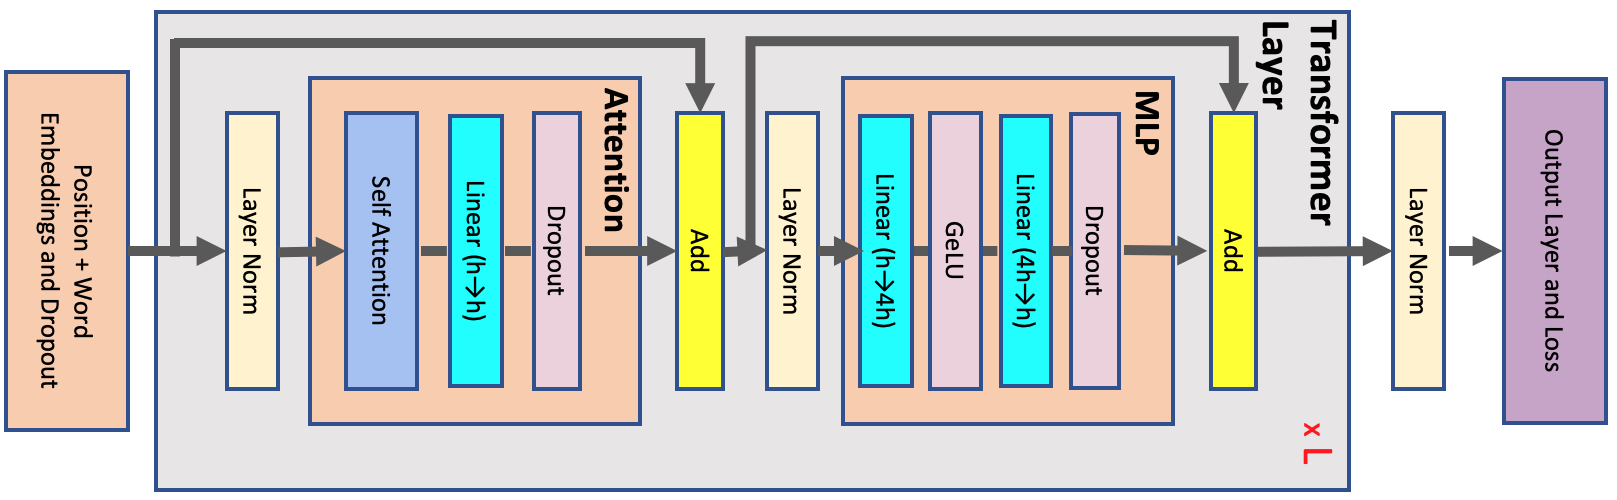
\includegraphics[scale=0.28]{figures/transformer-general.jpg}
	\caption{The full transformers architecture. Diagram taken from \cite{korthikanti2022reducing} }
	\label{fig_transformers_architecture}
\end{figure}

At a high level, decoder-only transformers take in an ordered series of word-like objects, called
tokens, and are trained to predict the next token in the sequence. Given some initial
text, transformers can be used to give a prediction for the likelihood of any possible continuation
of that text. An outline of the mechanics\footnote{This describes the vanilla architecture; almost
every component is modified in the available variants.}:
\begin{enumerate}
	\item Raw text is \textbf{tokenized} and turned into a series of integers\footnote{There are
		      about \href{https://github.com/ray-project/llm-numbers}{1.3 tokens per word}, on average.} whose values lie in \pyinline{range(V)}, with $ V $ the vocabulary
	      size.
	\item The tokenized text is chunked and turned into \pyinline{(B, S)}-shaped (batch size and
	      sequence length, respectively) integer tensors, $ x _{ bs } $.
	\item The \textbf{embedding layer} converts the integer tensors into continuous representations of shape
	      \pyinline{(B, S, D)}, $ z _{ bsd } $, with $ D $ the size of the hidden dimension.
	      \textbf{Positional encodings} have also been added to the tensor at this stage to help the
	      architecture understand the relative ordering of the text.
	\item The $ z _{ bsd } $ tensors pass through a series of transformer blocks, each of which has
	      two primary components:
	      \begin{enumerate}
		      \item In the \textbf{attention} sub-block, components of $ z _{ bsd } $ at different
		            positions ($ s $-values) interact with each other, resulting in another \pyinline{(B, S, D)}-shaped
		            tensor, $  z' _{ bsd } $.
		      \item In the \textbf{MLP} block, each position in  $ z' _{ bsd } $ is processed
		            independently and in parallel by a two-layer feed-forward network, resulting once more
		            in a \pyinline{(B, S, D)}-shaped tensor.
	      \end{enumerate}
	      Importantly, there are \textbf{residual connections} around each of these\footnote{This
		      gives rise to the concept of the \textbf{residual stream} which each transformer block reads
              from and writes back to repeatedly.} (the arrows in
              Fig.~\ref{fig_transformers_architecture}), meaning that the output of each block is
              added back to its original input.
	\item Finally, we convert the \pyinline{(B, S, D)}-shaped
	      tensors to \pyinline{(B, S, V)}-shaped ones, $ y _{ bsv } $. This is the role of
	      the \textbf{language model head} (which is often just the embedding layer used in an inverse
	      manner.)
	\item  The $ y _{ bsv } $ predict what the next token will be, i.e. $ x _{ bs+1 } $, having seen the \textbf{context}
          of the first $ s $ tokens in the sequence. Specifically, removing the batch index for
          simplicity, a \pyinline{Softmax}  of $ y _{ sv } $ gives the conditional probability $ p _{ sv
          } = P(t _{ s+1 }|t _{ s } \ldots t _ {0}) $ for the indicated series of tokens. Because of
          the chain rule of probability, these individual probabilities can be combined to form the
          probability that any sequence of tokens follows a given initial seed\footnote{In more
          detail, these probabilities are created by products: $ P(t _{ s+n } \ldots t _{ s+1}| t _{
          s } \ldots  t _{ 0 }) =P(t _{ s+n }| t _{ s+n - 1} \ldots  t _{ s } \ldots  t _{ 0}) \times
      \ldots  \times P(t _{ s+1 } | t _{ s } \ldots  t _{ 0 }) $.}.
\end{enumerate}


Each batch (the $ b $-index) is processed independently. We omitted \pyinline{LayerNorm} and
\pyinline{Dropout} layers above, as well as the causal mask; these will be covered below as we step
through the architecture in more detail.



\subsection{Embedding Layer and Positional Encodings \label{subsubsec_embedding_and_pe} }

The \textbf{embedding} layer is just a simple look up table: each of the \pyinline{range(V)} indices
in the vocabulary is mapped to a $ D $-dimensional vector via a large \pyinline{(V, D)}-shaped
table/matrix. This layer maps $ x _{ bs } \longrightarrow z _{ bsd } $. In \pyinline{torch}, this is
an \pyinline{nn.Embedding(V, D)} instance.

To each item in a batch, we add identical \textbf{positional encodings} to the vectors above with
the goal of adding fixed, position-dependent correlations in the sequence dimension which will
hopefully make it easier for the architecture to pick up on the relative positions of the inputs
\footnote{Positional encodings and the causal mask are the only components in the vanilla transformers
	architecture which carry weights with a dimension of size $ S $; i.e. they are the only parts that
	have explicit sequence-length dependence. A related though experiment: you can convince yourself
	that if the inputs $ z_{ bsd } $
	were just random noise, the transformers architecture would not be able to predict
	the $ s $-index of each such input in the absence of positional encodings. } This layer maps $ z _{
			bsd} \leftarrow z _{ bsd } + p _{ sd } $, with $ p _{ sd } $ the positional encoding tensor.

The above components require $ (V+S)D \approx VD $ parameters per model.



\subsection{Layer Norm \label{subsubsec_layer_norm} }

The original transformers paper \cite{vaswani2017attention} put \pyinline{LayerNorm} instances after
the \textbf{attention} and \textbf{MLP} blocks, but now it is common \cite{xiong2020layer} to put
them before these blocks\footnote{Which makes intuitive sense for the purposes of stabilizing the
	matrix multiplications in the blocks}.

The \pyinline{LayerNorm} operations acts over the sequence dimension. Spelling it out, given the
input tensor $ z _{ bsd } $ whose mean and variance over the $ s $-index are $ \mu _{ bd } $ and $
	\sigma _{ bd } $, respectively, the \pyinline{LayerNorm} output is
\begin{align}
	z _{ bsd } & \leftarrow \left ( \frac{ z _{ bsd } - \mu _{ bd } }{ \sigma _{ bd } } \right )\times \gamma _{ d }
	+ \beta _{ d } \equiv \LN _{ s } z _{ bsd}
\end{align}
where $ \gamma _{ d }, \beta  _{ d } $ are the trainable scale and bias parameters. In
\pyinline{torch}, this is a \pyinline{nn.LayerNorm(D)} instance.
Since there are two \pyinline{LayerNorm} instances in each transformer block, these components require
$ 2D $ parameters per layer.

We will continue discussing \pyinline{LayerNorm} instances in what follows in order to adhere to the
usual construction and to discuss methods like sequence-parallelism in their original form (see
Sec.~\ref{subsec_seq_parallelism}), but note: the data-independent \pyinline{LayerNorm}
transformations are completely redundant when immediately followed by a \pyinline{Linear} layer,
since both act linearly on their inputs and \pyinline{Linear} is already the most general
data-independent linear transformation. Explicitly, the  $ \gamma _{ d }, \beta _{ d } $ parameters
can be absorbed into the linear parameters as in
\begin{align}
	\left (     z _{ bsd } \gamma _{ d } + \beta _{ d } \right )  W _{d d'}    + b _{ d' } & = z _{ bsd }
	W' _{ d d' } + b' _{ d' } \ , \quad W' _{ d d' } \equiv  \gamma _{  d} W _{ d d' } \ , \quad b' _{
	d' } \equiv b _{ d' } + \beta _{ d }W _{ d d' } \ .
\end{align}
That is, these transformations can be equivalently performed by the weight matrix and bias (if
included) in \pyinline{Linear} layer\footnote{Note the importance of data-independence here: the
data-dependent subtraction of the mean and division by the standard deviation cannot be absorbed
for all elements in a batch.  Note that because the usual training algorithms are not covariant
under parameter redefinitions, the above unfortunately does not imply that removing
\pyinline{LayerNorm}s will have no effect on training dynamics.}.

\subsection{Causal Attention \label{subsubsec_attn_layer} }

\textbf{Causal attention} is the most complex layer. It features $ A $  sets of weight
matrices\footnote{There are also bias terms, but we will often neglect to write them explicitly or
    account for their (negligible)
	parameter count.}  $ Q  _{ d e a}, K  _{ de a}, V  _{ dea }  $
where $ a \in \left \{ 0, \ldots, A-1 \right \} $ and $ e \in \left \{ 0, \ldots, D/A \right \} $,
where $ D $ is assumed perfectly divisible by $ A $.
From these, we form three different vectors:
\begin{align}
	q _{ bsea } & = z _{ bsd } Q _{ dea } \ , \quad
	k _{ bsea } = z _{ bsd } K _{ dea }  \ , \quad
	v _{ bsea } = z _{ bsd } V _{ dea }
\end{align}
These are the \textbf{query, key, and value} tensors, respectively \footnote{There are of course
	many variants of the architecture and one variant which is popular in Summer 2023 is multi-query
	attention \cite{shazeer2019fast} in which all heads share \textit{the same} key and value vectors
	and only the query changes across heads, as this greatly reduces inference costs.}.

Using the above tensors, we will then build up an \textbf{attention map}  $ w _{ bss'a } $
which corresponds to how much attention the token at position $ s $ pays to the token at
position $ s' $.  Because we have the goal of predicting the
next token in the sequence, we need these weights to be causal: the final prediction $ y _{ bsv } $
should only have access to information propagated from positions $ x _{ bs'v } $ with $ s' \le s $.
This corresponds to the condition that $ w _{ bss'a} = 0  $ if  $ s' > s  $.

These weights come from \pyinline{Softmax}-ed attention scores, which are just a normalized
dot-product over the hidden dimension:
\begin{align}
    w _{ bss'da } & =\Sm _{ s' } \left (m _{ s s' }+\frac{q _{ bse }k _{ bs'ea } }{ \sqrt{D/A}}  \right
	)\ ,  \quad {\rm s.t.} \quad \sum_{s'}w _{ bdss'a } =1
\end{align}
The tensor $ m _{  s s' } $ is the causal mask which zeroes out the relevant attention map
components above
\begin{align}
	m _{ s s' } & = \begin{cases}
		                0       & s \le s' \nn
		                -\infty & = s > s'
	                \end{cases}\ ,
\end{align}
forcing $ w  _{ bss'da } =0$ for $ s> s' $. In other words, the causal mask ensures that a
given tensor, say $ z _{ bsd } $, only has dependence on other tensors whose sequence index, say $
	s' $, obeys $ s' \le s $.  This is crucial for inference-time optimizations, in particular the use
of the \textbf{kv-cache} in which key-value pairs do not need to be re-computed.

The $ \sqrt{D/A} $ normalization is motivated by demanding
that the variance of the \pyinline{Softmax} argument be 1 at initialization, assuming that other
components have been configured so that that the query and key components are i.i.d. from a Gaussian
normal distribution \footnote{However, in \cite{yang2022tensor} it is instead argued that no square
	root should be taken in order to maximize the speed of learning via SGD.}.

The weights above are then passed through a dropout layer and used to re-weigh the \textbf{value} vectors and form the tensors
\begin{align}
	y _{ bse a} & =\Dr  \left (w _{ bdss' a} \right ) v _{ bs'ea }
	\label{eq_reweighted_values}
\end{align}
and these \pyinline{(B, S, D/A, A)}-shaped tensors
are then concatenated along the $ e $-direction to re-form a \pyinline{(B, S, D)}-shaped
tensor $ u _{ bsd } $
\begin{align}
    u _{ bsd } & = y _{ bs(e a) }
\end{align}
in \href{https://einops.rocks/1-einops-basics/}{\pyinline{einops}}-like notation for concatenation.
Finally, another weight matrix $ O _{d' d } $ and dropout layer transform the output once again to get the final
output
\begin{align}
	z _{ bsd } & = \Dr \left (u  _{ bsd' } O _{ d'd }\right )\ .
\end{align}

For completeness, the entire operation in condensed notation with indices left implicit is:
\begin{align}
	z & \leftarrow \Dr \left ({\rm Concat} \ \left ( \Dr \left (\Sm  \left ( \frac{ \left ( z \cdot Q _{ a } \right )\cdot \left ( z \cdot K _{ a } \right )}{ \sqrt{D/A} }
		\right)\right )\cdot z \cdot V _{ a } \right ) \cdot O \right ) \label{eq_causal_attn}
\end{align}
where all of the dot-products are over feature dimensions (those of size $ D $ or $ D/A $).

Below is pedagogical\footnote{The
code is written for clarity, not speed. An example optimization missing here: there is no need to
form separate $ Q _{ a },K _{ a },V _{ a} $ \pyinline{Linear} layers, one large layer which is later
chunked is more efficient} sample code for such a  \pyinline{CausalAttention} layer\footnote{When
	using sequence-parallelism, it will be more natural to separate out the final \pyinline{Dropout} layer
	and combine it with the subsequent \pyinline{LayerNorm}, as they are sharded together; see
	Sec.~\ref{subsec_seq_parallelism}. The same is true for the \pyinline{MLP} layer below.}:
\pyfile[firstline=8,lastline=72]{python/causal_attention.py}

The parameter count is dominated by the weight matrices which carry $ 4 D ^{ 2 } $ total parameters
per layer.


\subsection{MLP \label{subsubsec_mlp} }

The feed-forward network is straightforward and corresponds to
\begin{align}
	z _{ bsd } & \leftarrow \Dr \left (\phi \left ( z _{ bsd' }W ^{ 0 }_{ d'e } \right ) W ^{ 1 } _{ ed
	} \right ) \label{eq_mlp}
\end{align}
where $ W ^{ 0 } $ and $ W ^{ 1 } $ are \pyinline{(D, ED)}- and \pyinline{(ED, D)}-shaped matrices,
respectively (see App.~\ref{app_conventions} for notation) and $ \phi $ is a
non-linearity\footnote{The \pyinline{GeLU}
	\href{https://pytorch.org/docs/stable/generated/torch.nn.GELU.html}{non-linearity} is common.}.
In code, where we again separate out the last \pyinline{Dropout} layer as we did in in
Sec.~\ref{subsubsec_attn_layer}.  \pyfile[firstline=6, lastline=27]{python/mlp.py}

This bock requires $ 2 E D ^{ 2 } $ parameters per layer, only counting the contribution from
weights.


\subsection{Language Model Head \label{subsubsec_language_model_head} }


The layer which converts the \pyinline{(B, S, D)}-shaped outputs, $ z _{ bsd } $, to \pyinline{(B, S, V)}-shaped
predictions over the vocabulary, $  y _{ bsv } $, is the \textbf{Language Model Head}. It
is a linear layer, whose weights are often tied to be exactly those of the initial embedding
layer of Sec.~\ref{subsubsec_embedding_and_pe}.


\subsection{All Together}
It is then relatively straightforward to tie everything together.  In code, we can first create a
transformer block like
\pyfile[firstline=8, lastline=45]{python/transformer_block.py}
which corresponds to the schematic function
\begin{align}
	z & \leftarrow  z + \texttt{MLP}\left ( \LN \left ( z + \texttt{CausalAttention}\left ( \LN \left (
				z\right ) \right )  \right ) \right )\ ,
\end{align}
indices suppressed.

And then the entire architecture: \pyfile[firstline=7, lastline=56]{python/decoder_only.py}


\subsection{The Loss Function}

The last necessary component is the loss function. The training loop data is the
\pyinline{(B, K)}-shaped\footnote{\pyinline{K} is the block size, the maximum sequence-length for
	the model. See App.~\ref{app_conventions}.}  token inputs ($ x _{ bs } $) along with their shifted-by-one relatives $ y
		_{ bs }$ where \pyinline{x[:, s + 1] == y[:, s]}.  The \pyinline{(B, K, V)}-shaped
outputs ($ z _{ bsv } $)  of the \pyinline{DecoderOnly} network are treated as the logits which
predict the value of the next token, given the present context:
\begin{align}
	p(x _{ b (s+1) }=v| x _{ b s }, x _{ b (s-1) }, \ldots, x _{ b 0 }) & = \Sm _{ v }\ z _{ bsv
		}\label{eq_transformer_conditional_prob}
\end{align}
and so the model is trained using the usual cross-entropy/maximum-likelihood loss
\begin{align}
	\Lcal & = -\frac{ 1 }{ BK }\sum _{ b,s }\ln p(x _{ b (s+1) }=y _{ b(s+1) }| x _{ b s }, x _{ b (s-1) },
	\ldots, x _{ b 0 })\nn
	      & = \frac{- 1 }{ BK }\sum _{ b,s }\Sm _{ v }\ z _{ bsv}\big| _{ v=y _{ b(s+1) } } \ .
\end{align}
Note that the losses for all possible context lengths are included in the sum, equally
weighted\footnote{In Natural Language Processing (NLP), the \pyinline{perplexity} is often reported
    instead of the loss, which is just the exponential of the loss, a geometric-mean over the
    gold-answer probabilities: $ {\rm perplexity} = e^{ \Lcal } =\left (\prod _{ b, s }p(x _{ b
        (s+1) }=| x _{ b s }, x _{ b (s-1) }, \ldots, x _{ b 0 })\right ) ^{ \frac{ -1 }{ BK } }$.}.

In \pyinline{torch}
code, the loss computation might look like the following (using fake data):
\pyfile[firstline=7, lastline=22]{python/loss.py}


\section{Architecture and Algorithm Variants}

There are, of course, many variants on the basic architecture. Some particularly important ones are
summarized here.


\subsection{Multi-Query Attention \label{subsec_multi_query_attn}}

In \cite{shazeer2019fast}, the $ A $ different key and value matrices are replaced by a single
matrix each, while $ A$ different query-heads remain. The mechanisms are otherwise unchanged: where
there were previously distinct key and value tensors used across different heads, we just use the same
tensors everywhere. This is \textbf{Multi-Query Attention} (MQA).


The primary reason for multi-query attention is that it vastly reduces the size of the kv-cache (see
Sec.~\ref{sec_kv_cache}) during inference time, decreasing the memory-burden of the cache by a
factor of $ A $. This strategy also reduces activation memory during training, but that is more of a
side-effect.

\subsection{Grouped Attention \label{subsec_grouped_attn}}

\textbf{Grouped Query Attention} (GQA) \cite{ainslie2023gqa} is the natural extension of
multi-query-attention to using $ 1<G<A $ matrices for key and value generation. Each of the $G$
different keys gets matched up with $A/G$ heads (nice divisibility assumed)\footnote{Llama-2
    \cite{touvron2023llama2} uses GQA with $ G=8 $, seemingly chosen so that each group can be
sharded and put on its own GPU within a standard 8-GPU node.}.


\subsection{Parallel \pyinline{MLP} and \pyinline{CausalAttention} Layers}

Rather than first pass inputs into the \pyinline{CausalAttention} layer of each block, and then pass
those outputs on to \pyinline{MLP} in series, \href{https://github.com/kingoflolz/mesh-transformer-jax/blob/f8315e3003033b23f21d78361b288953064e0e76/mesh_transformer/layers.py#L303}{GPT-J-6B}
instead processes the \pyinline{LayerNorm} outputs in \textit{parallel}. That is, instead of something
like
\begin{align}
	z \leftarrow z + \texttt{MLP}\left ( \texttt{LayerNorm}\left ( z + \texttt{CausalAttention}\left ( z \right ) \right ) \right )
\end{align}
we instead have\footnote{This alternative layer was also used in PaLM \cite{chowdhery2022palm} where it
	was claimed that this formulation is $\sim 15\%$ faster due to the ability to fuse the \pyinline{MLP}
	and \pyinline{CausalAttention} matrix multiplies together (though this is not done in the GPT-J-6B repo above).}
\begin{align}
	z \leftarrow z + \texttt{MLP}\left ( z \right )    + \texttt{CausalAttention}\left ( z \right )\ .
\end{align}
Note that a \pyinline{LayerNorm} instance is also removed.



\subsection{RoPE Embeddings}

A shortcoming of traditional embeddings $ x _{ bsd } \longrightarrow x _{ bsd } + p _{ sd } $ is
that they do not generalize very well: a model trained on such embeddings with a maximum sequence
length $ K $ will do very poorly when evaluated on longer sequences. RoPE (Rotary Position
Embedding) \cite{su2022roformer} and variants thereof can extend the viable context length by more
clever mechanisms with stronger implicit biases.

RoPE and its variants can be motivated by a few natural conditions.  Given the queries and keys for
an input $ q _{ sd }, k _{ sd } $ (suppressing batch indices), the corresponding attention scores
computation $ a _{ ss' }\left ( q _{ s }, k _{ s' } \right ) $ should reasonably satisfy the below:
\begin{enumerate}
	\item The attention score should only depend on the position indices $ s, s' $ through their difference
	      $ s-s' $, i.e., through their relative distance to each other.
	\item The score computation should still be efficient, i.e., based on matrix-mulitiplies.
	\item The operation should preserve the scale of the intermediate representations and attention
	      scores, in order to avoid issues with standard normalization.
\end{enumerate}
These conditions suggest a very natural family of solutions: rotation of the queries by some fixed
element of $ SO(d) $ with a generator proportional to the position index, and rotation of keys by
the conjugate element,
\begin{align}
	q _{ sd } & \longrightarrow \left [e^{ i s \hat{n}\cdot T }\right ]_{ d d' } q _{ sd' } \equiv R(s) _{ d d' } q _{ sd' } \nn
	k _{ sd } & \longrightarrow \left [e^{ -i s \hat{n}\cdot T }\right ]_{ d d' } k _{ sd' } \equiv  R(s)^{ \dagger } _{ d d' } k _{ sd' } \ . \label{eq_rope}
\end{align}

Performing the above computation with a dense element of $ SO(D) $ is infeasible, as it would require
a new dense matrix-multiply by a unique $ D \times D $ matrix at each sequence
position\footnote{For one, the $ \Ocal \left( SD ^{ 2 } \right)  $ memory cost to store the matrices
    would be prohibitive. The FLOPs cost is only $ 2BSD ^{ 2 } $, the same as for other matrix
    multiplies, but because different matrices are needed at position, these FLOPs would be much more
    GPU memory-bandwidth intensive.
}

In the original RoPE paper, the rotation $ \hat{n} $ was chosen such that the matrices are $ 2
	\times  2 $ block-diagonal with the entries of the form\footnote{If $ D $ isn't even, the vectors
	are padded by an extra zero.}
\begin{align}
	R(s)_{ [d:d+2][d:d+2] } & =\begin{pmatrix}
		                           \cos \left ( s \theta _{ d }   \right ) & -\sin \left ( s \theta _{ d }   \right ) \\
		                           \sin \left ( s \theta _{ d }   \right ) & \cos \left ( s \theta _{ d }   \right )
	                           \end{pmatrix}
\end{align}
where
\begin{align}
	\theta _{ d } & = 10 ^{ -8d/D   } \ .
\end{align}
The RoPE memory costs are thus $ \Ocal \left( K D \right)  $\footnote{A single RoPE buffer can be
shared amongst all attention layers, amortizing the memory costs.}. The sparsity present in this constrained form of the RoPE matrices means that
\eqref{eq_rope} can be computed in $ \Ocal \left( BSD \right)  $ time, rather than $ \Ocal \left(
BSD ^{ 2 } \right)$, as it would be for a general rotation matrix. See the paper for explicit
expressions.


\subsection{Flash Attention \label{subsec_flash_attention}}


Flash Attention \cite{dao2022flashattention, dao2023flashattention2} optimizes the self attention
computation by never materializing the $ \Ocal \left( S ^{ 2 } \right)  $ attention scores in
off-chip memory. This increases the arithmetic intensity of the computation and reduces the
activation memory required, at the expense of needing recomputation in the backwards pass.


The central idea is to decompose the attention computation in the following way. Dropping the batch
index, let $ q _{ sd }, k _{ sd }, v _{ sd } $ be the queries, keys, and values, and $ z _{ sd } $
be the final output. Splitting into attention heads as in $ q _{ sd } = q _{ s(ah) }\longrightarrow q _{ sah } $
and similar the computation is
\begin{align}
    z _{ sah } &= \Sm _{ s' } \left ( q _{ sah' } k _{ s'ah' } \right ) v _{ s'ah }
\end{align}
which is then concatenated as $ z _{ s(ah) }\longrightarrow  z _{ sd } $ to get the result.

The $ \Ocal \left( A S ^{ 2 } \right)  $ attention scores $ \Sm _{ s' } \left ( q _{ sah' } k _{
s'ah' } \right ) $ are expensive to shuttle back and forth from off-chip to on-chip memory and are a
costly activation memory component. To this end, Flash Attention functions by further chunking $ q,
z $ over the sequence dimension as in $ q _{ sd }= q _{ (ir)(ah) }\longrightarrow  q _{ airh }  $,
and similar for $ z $, and $ k,v $ where $ k _{ sd }= k _{ (jc)(ah) }\longrightarrow  k _{ ajch }
$, and similar for $ v $. The chunk sizes are such that the attention scores for each chunk can be
computed with minimal off-chip operations (by using shared memory), which is where the performance
gains come from. With this splitting, the above reads
\begin{align}
    z _{ irah } &= \Sm _{ j'c' } \left ( q _{ irah' } k _{ j'c'ah' } \right ) v _{ j'c'ah } \nn
     &= P _{ irj'c'a } v _{ jc'ah } \label{eq_flash_attn_sums}
\end{align}
where range of the new indices is dictated by the available on-chip memory and is analyzed below.

The algorithm functions by performing the sums in \eqref{eq_flash_attn_sums} on-chip, meaning that
neither the attention scores (Softmax inputs) nor the probabilities ever need to be shuttled back
and forth. We will jump right to the second version of the algorithm.   In addition to
the final outputs $ z _{ irah } $, the algorithm saves the Softmax denominators $ \ell
_{ ira } $ ($ AS $ total elements) which are related to the softmax probabilities as in
\begin{align}
    P _{ irjca } &= \frac{  \exp \left (   q _{ irah } k _{ jcah }\right)}{ \ell _{ ira } } \ .
\end{align}
Because only the Softmax outputs $ P $ are needed to compute the Softmax derivative
\eqref{eq_softmax_derivative}, we can use the $ \ell _{ ira} $ to compute the backwards pass if we
also recompute the exponential term.


The entire forward-pass algorithm is as follows. Essentially, one just computes partial values for
each term in the softmax sum, correcting old results and adding new terms to the sum with each
iteration. We capitalize tensors which only exist on-chip and leave tensors which come from off-chip
lower-cased. The entire $ z _{ irah } $ tensor is then computed as (we omit the attention head $ a
$-index for clarity):
\begin{algo}{Flash Attention Version Two (Forward)}
\For{ $ i \in \ldots  $}
\State Initialize off-chip tensors $ z _{ irh },  \ell _{ ir }$ to zeros
\State Move  $ q _{ irh }$ on-chip, instantiate $Z _{ ijrh }, L _{ ijr }$ to zeros and $M _{ ijr }$ to $ -\infty $ on-chip.
\For{ $ j \in \ldots  $}
    \State Move  $ k_{ jch' },v _{ jch' }$ on-chip
    \State $ S _{ irjc } \gets q _{ irh' } k _{ jch' } $  \Comment $ S _{ irjc } $ is a temp, only needed for one $ i,j $ iter
    \State $ M _{ irj }  \gets \max(M _{ i(j-1)r },  \max _{ c } S _{ irjc } ) $ \Comment Get max attention score seen so far
    \State $ \tilde{P} _{ irjc} \gets \exp \left ( S _{ irjc } - M _{ irj } \right ) $
    \State $ L _{ irj }  \gets e^{ M _{ i(j-1)r } - M _{ irj }}L _{ irj } + \sum _{ c }\tilde{P} _{ irjc }$ \Comment Correct, update denominators
    \State $ Z _{ irjh } \gets   e^{ M _{ i(j-1)r } - M _{ irj } }Z _{ irjh } +\tilde{P} _{ irjc}v _{ jch }$ \Comment Correct, update numerators
\EndFor
\State $ z _{ irh } \gets \frac{1}{L _{ i(-1)r }} Z _{ i(-1)rh }$ \Comment Divide $ z $ by last $ j  $ value of $ L _{ ijc } $
    \State $ \ell _{ ir } \gets M _{ i(-1)r }+\ln L _{ i(-1)r }$ \Comment Store statistics for bwd
    \State Write  $z _{ irh } ,  \ell _{ ir }$ to off-chip memory
\EndFor
\label{algo_fa_v2}
\end{algo}

The application of the causal mask is not shown. The for-loop just unrolls the $ j' $ sum in
\eqref{eq_flash_attn_sums}.



 Whereas vanilla attention requires $ \Ocal \left( S ^{ 2 }+ DS \right)  $ memory transfers per
 attention head, flash attention requires fewer. Let $ M $ be the amount of on-chip memory in bytes
 and let $ R  $ be the range of $ r \in \left \{ 0, \ldots , R-1 \right \} $ and similar for other
 indices. Being able to to fit all of the necessary tensors in on-chip memory requires $ CH + RH +
 RC \lesssim \Ocal \left( M \right)  $.  Most of the memory transfers above come from the $k, v$
 accesses in the inner loop, which access $ \Ocal \left( \frac{ HS ^{ 2 } }{ R } \right)$ elements
 over the lifetime of the algorithm. Assuming the chunks were chosen to maximize on-chip memory
 usage, such that $ RH \sim \Ocal \left( M \right)  $, this is  $  \Ocal \left(\frac{ H ^{ 2}S ^{ 2
 } }{ M }  \right) $ bytes of memory. Since $ M \sim 10 ^{ 5 } $ bytes on 2023 GPUs, this is fewer
 than $ \Ocal \left( S ^{ 2 } \right) $ access for the typical  head dimensions  $ H \lesssim 10 ^{ 2 }
 $.


Flash attention is also a big win for activation memory: a naive algorithm has a $ \Ocal \left( ABS
^{ 2 } \right)  $ per-layer contribution to activation memory due to needing to save the attention
weights, but these are discarded and re-computed for flash attention.  The only additional memory
cost comes from the $ \Ocal \left( ABS \right)  $ elements in the $ \ell _{ abs } $ statistics, which are
dominated by the $ \Ocal \left( BSD \right)  $ costs from needing to save inputs, and hence negligible.

\newpage

\part{Training}

\section{Memory \label{sec_memory_training}}

In this section we summarize the train-time memory costs of Transformers under various training
strategies\footnote{A nice related blog post is \href{https://blog.eleuther.ai/transformer-math/}{here}. \label{foot_eleuther_math_101} }.

The memory cost is much more than simply the cost of the model
parameters. Significant factors include:
\begin{itemize}
	\item Optimizer states, like those of \pyinline{Adam}
	\item Mixed precision training costs, due to keeping multiple model copies.
	\item Gradients
	\item Activation memory\footnote{Activations refers to any intermediate value which needs to be
		      cached in order to compute backpropagation. We will be conservative and assume that the inputs
		      of all operations need to be stored, though in practice gradient checkpointing and recomputation
		      allow one to trade caching for redundant compute. In particular, flash attention
		      \cite{dao2022flashattention} makes use of this strategy.} , needed for backpropagation.
\end{itemize}
Because the activation counting is a little more involved, it is in its own section.


\begin{nicebox}{Essentials}
	Memory costs count the elements of all tensors in some fashion, both from model parameters and
	intermediate representations. The gradient and optimizer state costs scale with the former quantity:
	$ \Ocal \left ( N _{ {\rm params}  } \right ) \sim \Ocal \left ( L D ^{ 2 } \right )$, only counting
	the dominant contributions from weight matrices. Activation memory scales with the latter,
	which for a \pyinline{(B, S, D)}-shaped input gives $ \Ocal \left ( BDLS  \right ) $ contributions
	from tensors which preserve the input shape, as well as $ \Ocal \left( ABLS ^{ 2 } \right)  $
	factors from attention matrices.
\end{nicebox}


\subsection{No Sharding}

Start with the simplest case where there is no sharding of the model states. Handling the different
parallelism strategies later will be relatively straightforward, as it involves inserting just a few
factors here and there.

\subsubsection{Parameters, Gradients, Optimizer States, and Mixed Precision
	\label{sec_params_grads_optim_mem}}


Memory from the bare parameter cost, gradients, and optimizer states are fixed costs independent of
batch size and sequence-length (unlike activation memory), so we discuss them all together here. The
parameter and optimizer costs are also sensitive to whether or not mixed-precision is used, hence we
also address that topic, briefly.  We will assume the use of \pyinline{Adam}\footnote{Which stores
	\href{https://pytorch.org/docs/stable/generated/torch.optim.Adam.html}{two different running
		averages} per-model parameter.} throughout, for simplicity and concreteness. It will sometimes be
useful below to let $ p $ to denote the precision in bytes that any given element is stored in, so
\pyinline{torch.float32} corresponds to $ p=4 $, for instance. Ultimately, we primarily consider
vanilla training in $ p=4 $ precision and \pyinline{torch.float32}/\pyinline{torch.float16} ($ p=4
$/ $ p=2 $)  mixed-precision, other, increasingly popular variants to exist, so we keep the
precision variable where we can.


Without mixed precision, the total cost of the
\pyinline{torch.float32} ($ p=4 $ bytes) model and optimizer states in bytes is then
\begin{align}
	M _{ \rm model} & = 4 N _{ \rm params } \ , \quad M_{ \rm  optim } = 8 N _{ \rm params }
	\quad ({\rm no \ mixed \ precision, } p=4)
	\label{eq_optimizer_states_mem_no_mp}
\end{align}
where, from the previous section, the pure parameter-count of the decoder-only Transformers
architecture is
\begin{align}
	N _{ \rm params } & \approx  (4 + 2E) L D ^{ 2 } \times \left ( 1 + \Ocal \left( \frac{ V }{ DL }
		\right) + \Ocal \left( \frac{ 1 }{ D } \right)  \right ) \ . \label{eq_approx_params_no_sharding}
\end{align}
where the first term comes from the \pyinline{TransformerBlock} weight matrices\footnote{So,
	in the usual $ E=4 $ case, the \pyinline{MLP} layers are twice as costly as the
	\pyinline{CausalAttention} layers.}, the first omitted subleading correction term is the embedding
matrix, and the last comes from biases, \pyinline{LayerNorm} instances, and other negligible
factors.  The optimizer states cost double the model itself.


The situation is more complicated when mixed-precision is used \cite{micikevicius2018mixed}.
The pertinent components of mixed-precision\footnote{A note on the implementation of mixed-precision
in \pyinline{torch}: usually mixed-precision occurs by wrapping the forward pass in a context
manager, \pyinline{torch.autocast}. The default behavior is to then create copies of some tensors
in lower-precision and do the forward pass with those. For instance, this is done with
matrix-multiplies whose arguments and outputs will be in \pyinline{torch.float16}, but for sums
the inputs and outputs will all be \pyinline{torch.float32}, for vanilla mixed-precision usage.
Consequently, any such \pyinline{torch.float16} versions of tensor will often persist effectively
as contributors to activation memory, since the backwards pass will need those same tensors. This
can be verified by inspecting the saved tensors: if \pyinline{z} is the output of a
matrix-multiply in such an autocast context, \pyinline{z.grad_fn._saved_mat2} will be a
\pyinline{torch.float16} copy of the weights used to perform the matrix-multiply. In effect, the
cost of the model weights which are used for the actual forward pass are only materialized within
the lifetime of the context manager.}:
\begin{itemize}
	\item A half-precision ($ p=2 $ bytes) copy of the model is used to perform the forwards and
	      backwards passes
	\item A second, "master copy" of the model is also kept with weights in full $ p=4 $ precision
	\item The internal \pyinline{Adam} states are kept in full-precision
\end{itemize}
Confusingly, the master copy weights are usually accounted for as part of the optimizer state, in
which case the above is altered to
\begin{align}
	M _{ \rm model} & = 2 N _{ \rm params } \ , \quad M_{ \rm  optim } = 12 N _{ \rm params }
	\quad ({\rm mixed \ precision}) .
	\label{eq_optimizer_states_mem_mp}
\end{align}
The optimizer state is now six times the cost of the actual model used to process data and the costs
of \eqref{eq_optimizer_states_mem_mp} are more than those of \eqref{eq_optimizer_states_mem_no_mp}.
However, as we will see, the reduced cost of activation memory can offset these increased costs, and
we get the added benefit of increased speed due to specialized hardware. The above also demonstrates
why training is so much more expensive than inference.


\subsubsection{Gradients}

Gradients are pretty simple and always cost the same regardless of whether or not mixed-precision is
used:
\begin{align}
	M_{ \rm grad} & = 4 N _{ \rm params }     \label{eq_grad_memory} \ .
\end{align}
In mixed precision, even though the gradients are initially computed in $ p= 2$, they
\href{https://huggingface.co/docs/transformers/v4.20.1/en/perf_train_gpu_one#anatomy-of-models-memory}{have to
	be converted} to $ p=4 $ to be applied to the master weights of the same precision.




\subsubsection{Activations}

Activations will require a more extended analysis \cite{korthikanti2022reducing}. Unlike the above
results, the activation memory will depend on both the batch size and input sequence length, $ B $
and $ S $, scaling linearly with both.



\paragraph{Attention Activations}

We will count the number of input elements which need to be cached. Our \pyinline{(B, S, D)}-shaped inputs
to the attention layer with $ BDS $ elements are first converted to $ 3BDS $ total query, key, value
elements, and the query-key dot products produce $ ABS ^{ 2 } $ more, which are softmaxed into $ ABS
		^{ 2 } $ normalized scores. The re-weighted inputs to the final linear layer also have $ BDS $
elements, bringing the running sum to $ BS \left ( 5D + 2AS  \right ) $

Finally, there are also the dropout layers applied to the normalized attention scores and the final
output whose masks must be cached in order to
backpropagate. In torch, the mask is a \pyinline{torch.bool} tensor, but
\href{https://github.com/pytorch/pytorch/issues/41571}{surprisingly} these use one \textit{byte} of
memory per element, rather than one bit \footnote{As you can verify
	via \pyinline{4 * torch.tensor([True]).element_size() == torch.tensor([1.]).element_size().}}.
Given this, the total memory cost from activations is
\begin{align}
	M _{ \rm act  } ^\texttt{Attention} & = BLS \left ( (5p+1)D + (2p+1)AS  \right ) \ .
	\label{eq_att_actmem_vanilla}
\end{align}




\paragraph{MLP Activations}

First we pass the \pyinline{(B, S, D)}-shaped inputs into the first MLP layer. These turn into the
\pyinline{(B, S, E*D)} inputs of the non-linearity, whose same-shaped outputs are then passed into
the last \pyinline{Linear} layer, summing to $ (2E+1)BDS $ total elements thus far. Adding in the
dropout mask, the total memory requirement across all \pyinline{MLP} layers is:
\begin{align}
	M _{ \rm act  } ^\texttt{MLP} & = (2Ep+p+1)BDLS\ .
	\label{eq_mlp_actmem_vanilla}
\end{align}




\paragraph{LayerNorm, Residual Connections, and Other Contributions}

Then the last remaining components. The \pyinline{LayerNorm} instances each have $ BDS $ inputs and
there are two per transformer block, so $ M _{ {\rm  act}  } ^\texttt{LayerNorm} = 2pBDLS $, and
there is an additional instance at the end of the architecture\footnote{Following
\cite{korthikanti2022reducing} we will neglect this in the below sum, an $ \Ocal \left( 1/L
\right) $ error}. There are two residual connections per block, but their inputs do not require
caching (since their derivatives are independent of inputs). Then, there are additional
contributions from pushing the last layer's outputs through the language-model head and
computing the loss function, but these do not scale with $ L $ and are ultimately $ \sim \Ocal
\left( \frac{ V }{ DL } \right)  $ suppressed, so we neglect them.





\paragraph{Total Activation Memory}


Summing up the contributions above, the total activation memory cost per-layer is
\begin{align}
	M _{ {\rm act}  } ^{ {\rm  total}  } & \approx  2BDLS   \left ( p(E+4) + 1 + \Ocal \left( \frac{
		V}{ DL } \right)  \right )
	+ ABLS ^{ 2 } \left ( 2p+1\right ) \label{eq_act_mem_total_no_sharding}\ .
\end{align}
Evaluating in common limits, we have:
\begin{align}
	M _{ {\rm act}  } ^{ {\rm  total}  } \Big| _{ E=4, p=4 } & =BLS \left ( 66 D+15AS  \right ) \nn
	M _{ {\rm act}  } ^{ {\rm  total}  } \Big| _{ E=4, p=2 } & =BLS \left ( 34 D+5AS  \right )
\end{align}


\paragraph{When does mixed-precision reduce memory?} (Answer: usually.) We saw in Sec.~\ref{sec_params_grads_optim_mem}
that mixed precision \textit{increases} the fixed costs of non-activation memory, but from the above
we also see that it also \textit{reduces} the activation memory and the saving increase with larger
batch sizes and sequence lengths. It is straightforward to find where the tipping point is.
Specializing to the case $E=4$, vanilla mixed-precision case with no parallelism\footnote{With both
	tensor- and sequence-parallelism, the parallelism degree $ T $ actually drops out in the comparison
	(since both form of memory are decrease by $ 1/T $, so this restriction  can be lifted.}, the
minimum batch size which leads to memory savings is
\begin{align}
	B _{ {\rm min}  } & = \frac{ 6 D ^{ 2 } }{ 8 DS + A S ^{ 2 } }\label{eq_min_mp_batch_size}\ .
\end{align}
Plugging in numbers for the typical $ \Ocal \left( 40 \ {\rm GiB} \right)$ model in the Summer of
2023 gives $ B _{ {\rm min} } \sim \Ocal \left( 1\right)  $, so mixed-precision is indeed an overall
savings at such typical scales.



\begin{commentbox}{Side Note: Optimizations}

The above analysis is conservative and accounts for more tensors than are actually saved in
practice.\newline

For instance, both the input and outputs of all non-linearities were counted, but there are many
activations whose derivatives can be reconstructed from its outputs alone: $ \phi'(z)=F \left (
\phi(z) \right ) $ for some $ F $. Examples:
\begin{itemize}
    \item \pyinline{ReLU}: since $ \phi(z)= z\theta(z) $, then (defining the derivative at zero to
        be zero) $ \phi'(z) =\theta(z) = \theta \left ( \phi(z) \right) $. Correspondingly, torch
        only uses the \pyinline{ReLU} outputs \href{https://github.com/pytorch/pytorch/blob/73d288fdf9d0beb76229cabc8566ee116f8a21a2/tools/autograd/derivatives.yaml#L2009-L2011}{to compute the derivative}
        (there is no self arg in the \pyinline{threshold_backward(grad, result, 0)} line).
    \item  \pyinline{tanh}: since $ \tanh'(z)=1-\tanh(z) ^{ 2 } $.
\end{itemize}
Other cases do not have this nice property, in which case both the inputs and outputs need to
be stored:
\begin{itemize}
    \item \pyinline{GeLU} \cite{hendrycks2023gaussian}: $ \phi(z)=z\Phi(z) $ here and the derivative
        $ \phi'(z)= \Phi(z) + \frac{ z e^{ -z ^{ 2 } /2 } }{\sqrt{2\pi}  } $, both the inputs and
        outputs \href{https://github.com/pytorch/pytorch/blob/73d288fdf9d0beb76229cabc8566ee116f8a21a2/tools/autograd/derivatives.yaml#L2041-L2044}{must be used in the backwards pass.}.

        The explicit CUDA kernel \href{https://github.com/pytorch/pytorch/blob/73d288fdf9d0beb76229cabc8566ee116f8a21a2/aten/src/ATen/native/cuda/ActivationGeluKernel.cu#L70-L84}{is here}.
\end{itemize}
If the inputs in each of these cases are not needed for any other part of the backwards pass, they
are garbage collected in \pyinline{torch} soon after creation.


\paragraph{Example}: \pyinline{Softmax} is another instance where this occurs, since
\begin{align}
     \partial _{ i } \Sm \left ( x _{ j } \right )  &= \delta _{ ij }\Sm \left ( x _{ j } \right ) -   \Sm \left ( x _{ i } \right )  \Sm \left ( x _{ j } \right ) \label{eq_softmax_derivative}
\end{align}
Because of this, the actual amount of activation memory due to the attention layer after the
forwards pass is \eqref{eq_att_actmem_vanilla} with $ 2p \longrightarrow p $ in the $ \Ocal \left( S
^{ 2 } \right)  $ term, though the above expression better reflects the necessary peak memory.

\end{commentbox}

\subsection{Tensor Parallelism \label{subsec_tensor_parallelism} }

\begin{commentbox}{Side Note: }
    I wrote a blog post on this \href{https://www.determined.ai/blog/tp}{here.}
\end{commentbox}


In \textbf{Tensor Parallelism}, sometimes also called \textbf{Model Parallelism}, individual weight
matrices are split across devices \cite{shoeybi2020megatronlm}. We consider the \pyinline{MLP} and
\pyinline{CausalAttention} layers in turn. Assume $ T $-way parallelism such that we split some
hidden dimension into $ T $-equal parts across $ T $ workers\footnote{All $ T $ workers work on
    processing the same batch collectively.  With $ N>T $ workers, with $ N $ perfectly divisible by
    $ T $, there are $ N/T $ different data parallel groups. Critical-path TP communications occur
    within each data parallel group and gradients are synced across groups. Ideally, all the workers
    in a group reside on the same node, hence the usual $ T=8 $.}


\begin{nicebox}{Essentials}
	The cost of large weights can be amortized by first sharding its output dimension, resulting in
	differing activations across group members. Later, the activations are brought back in sync via
	a \pyinline{AllReduce}. Weights which act on the sharded-activations can also be sharded in their
	input dimension. In the backwards pass, another \pyinline{AllReduce} is required.
\end{nicebox}

\paragraph{MLP}
It is straightforward to find the reasonable ways in which the weights can be partitioned. We
suppress all indices apart from those of the hidden dimension for clarity.

The first matrix multiply $ z _{ d }W ^{ 0 } _{ d e } $ is naturally partitioned across the output
index, which spans the expanded hidden dimension $ e\in \left \{ 0, \ldots , ED-1 \right \} $. This
functions by splitting the weight matrix across its output indices across $ T $ devices:  $ W ^{ 0 }
_{ d e }= W ^{ 0 }_{ d (f t) } \equiv  \bar{W} ^{ 0 } _{ d f \bar{t} }$ (again in
\pyinline{einops}-like notation, with bars denoting that the tensor and particular indices are
sharded; see App.~\ref{app_conventions}), where in the split weights $ \bar{t}\in \left \{ 0, \ldots
, T-1 \right \} $, and $ f \in \left \{ 0, \ldots , \frac{ ED }{ T } -1\right \} $. Each of the $ T
$ workers compute one shard of $ z _{ d }\bar{W} ^{ 0 }_{ df \bar{t} } $, i.e. each has a different
value of $ \bar{t} $.


Let the partial outputs from the previous step be $ \bar{z} _{ ft }  $ (batch-index suppressed),
which are \pyinline{(B, S, E*D/T, T)}-shaped, with the final dimension sharded across workers. The
non-linearity $ \phi $ acts element wise, and using the updated $ \bar{z} _{ f \bar{t} }   $ to
compute the second matrix multiply requires a splitting the weights as in $ W ^{ 1 } _{ e d' }= W ^{
1 }_{ (ft)d' } \equiv \bar{W} ^{ 1 } _{  f \bar{t} d'}$ (dividing up the incoming $ e $ dimension),
such that the desired output is computed as in $  \bar{z} _{ f \bar{t} }\cdot \bar{W} ^{ 1 }_{ f
\bar{t}d' }$, sum over $ \bar{t} $ implied. Each device has only $\bar{t} $ component in the sum (a
\pyinline{(B, S, D)}-shaped tensor) and an \pyinline{AllReduce} is used to give all workers the
final result. This \pyinline{AllReduce} is the only forward-pass collective
communication\footnote{The amount of communicated data is $ \Ocal \left( BSD \right)$.}.

One-line summary of the parallel decomposition:
\begin{align}
 z _{ sd' } \leftarrow   \phi \left (z _{ d }W ^{ 0 }_{ de }\right )W ^{ 1 } _{ ed' } &=\phi \left (z _{ d }\bar{W} ^{ 0 }_{ df \bar{t} }\right )\bar{W} ^{ 1 } _{ f \bar{t}d' } \ .
\end{align}
The progression of tensor shapes held by any single worker is
\begin{enumerate}
    \item \pyinline{(B, S, D)}
    \item \pyinline{(B, S, E*D/T)}
    \item \pyinline {(B, S, D)}
\end{enumerate}

In the backwards pass, another \pyinline{AllReduce} (see App.~\ref{app_collective_communications})
is needed for proper gradient computations with respect to the first \pyinline{Linear} layer's
outputs. This is true whenever an operation producing a sharded output involved non-sharded tensors:
if an operation $ \bar{y}_{ \bar{r} }  = F(x, \ldots) $ produces a sharded output from an unsharded
in put $ x $ (all other indices suppressed), the derivative with respect to $ x $ requires a sum
over ranks, $ \frac{ \partial \Lcal }{ \partial x } = \frac{ \partial \Lcal }{ \partial \bar{y} _{
\bar{r} }  } \frac{ \partial \bar{y} _{ \bar{y} } }{ \partial x  }$. Note that each worker will have
to store all components of the input $ z $ for the backward pass.



\begin{figure}[ht]
	\centering
	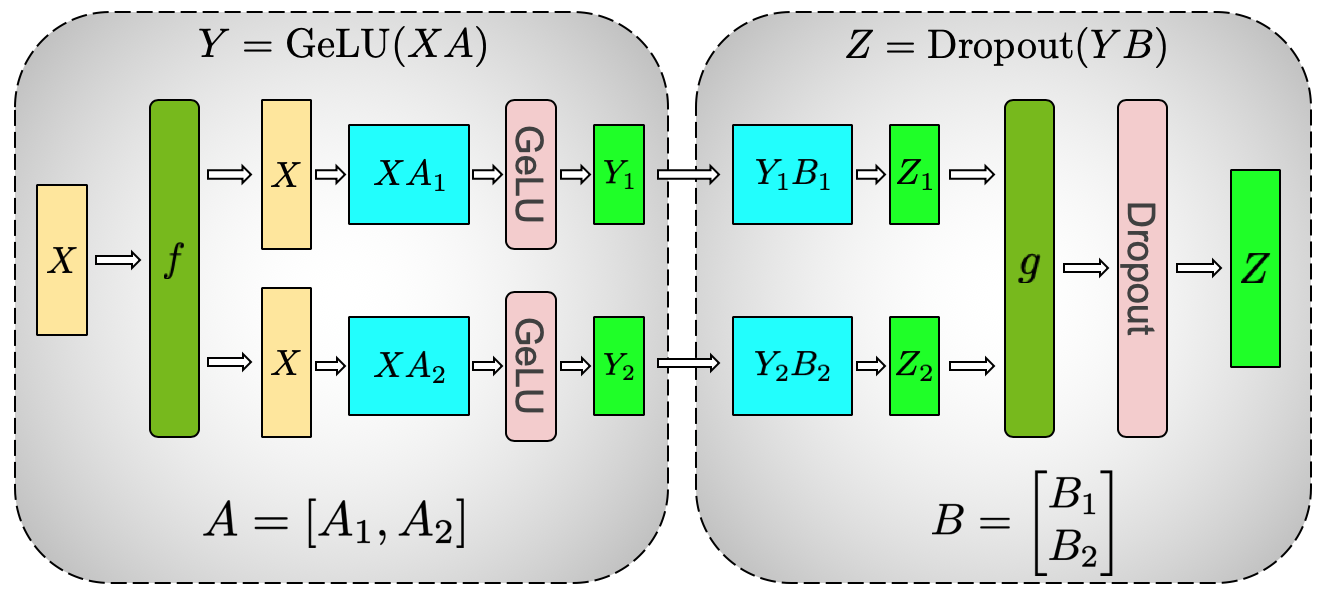
\includegraphics[scale=.33]{figures/mlp_mp_2.png}
	\caption{Tensor parallelism for the \pyinline{MLP} layers. Graphic from
		\cite{shoeybi2020megatronlm}. The $ f/g $ operations are the collective
		identity/\pyinline{AllReduce} operations in the forwards pass and the \pyinline{AllReduce}/identity
		operations in the backwards pass.}
	\label{fig_mlp_tensor_parallel}
\end{figure}


\paragraph{Attention} Because the individual attention head computations are independent, they can
be partitioned across $ T $ workers without collectively communications.  An \pyinline{AllReduce} is
needed for the final projection, however, which results in the various re-weighted values $ y _{
bsea } $ \eqref{eq_reweighted_values}.

To review, the attention outputs $ z' _{ sd } $ generated from inputs $ z_{ sd } $ can be expressed
as
\begin{align}
    z' _{ sea }  &= {\rm  MHA}(q _{ sea }, k _{ sea }, v _{ sea }) O _{ ead }\nn
\end{align}
where:
\begin{itemize}
    \item  We have split the $ d $-index as in $ z _{ sd }\longrightarrow z _{ s (ea) } $ with $ e $ and
$ a $ the head-dimension and head-index
    \item $ q _{ sea }, k _{ sea }, v _{ sea }
$ are the query, keys and values derived from the inputs
    \item ${\rm
    MHA } $ is the multi-head attention function, whose outputs are the same shape as its value inputs
    \item The dual sum over head-dimension index ($ e $) and attention-head-index ($ a $) is the
    sum-and-concatenate step from the more explicit description in Sec.~\ref{subsubsec_attn_layer}
    \item \pyinline{Dropout} and biases were ignored for simplicity
\end{itemize}

In order to parallelize the above $ T $-ways, we simply shard across the dimension $ a $  which
indexes the different attention heads.  The $ {\rm MHA} $ computations all process in
embarassingly-parallel fashion, and an all-reduce is needed to complete the sum over the $ a $-index
across devices.

The collective communications story is essentially
equivalent to that of the \pyinline{MLP} layers\footnote{The amount of communicated data is again $ \Ocal \left( BSD
\right)$. }: one \pyinline{AllReduce} is needed in the forwards pass
and one \pyinline{AllReduce} in the backwards-pass.

The progression of tensor shapes held by any single worker is
\begin{enumerate}
    \item \pyinline{(B, S, D)}
    \item \pyinline{(B, S, D/A, A/T)}
    \item \pyinline {(B, S, D)}
\end{enumerate}


It is worth comparing the communications and FLOPs costs of these sharded layers. Each layer costs
$ \Ocal \left(    BS \left ( 4+2E \right )  D ^{ 2 }/T \right)$ FLOPs and communicates
$ \Ocal \left( BSD \right)  $ bytes and so the communication-to-compute-time ratio is
\begin{align}
  \frac{ t _{ {\rm  compute} } }{ t _{ {\rm  comms} } } & \sim  \frac{ \left ( 4+2E \right) D }{ T }\times \frac{ \lambda _{ {\rm comms} }  }{ \lambda _{ {\rm FLOP/s} }} \ .
\end{align}
Since\footnote{Assuming $ \lambda _{\rm  FLOP/s }\sim  $100 TFLOP/s and $ \lambda _{ {\rm comms} }
\sim $ 100 GiB/s.} $ \frac{ \lambda _{ {\rm comms} }  }{ \lambda _{ {\rm FLOP/s} }} \sim 10 ^{ -3 }
$FLOPs/B, communication and compute take similar times when  $ D \sim \Ocal \left( 10 ^{ 3 } \right)
$ for typical setups with $ T \sim \Ocal \left( 10 \right)  $ and so tensor-parallelism requires
$ D \gtrsim 10 ^{ 4 } $ to reach similar efficiency to the non-tensor-parallel implementations.


\begin{figure}[ht]
	\centering
	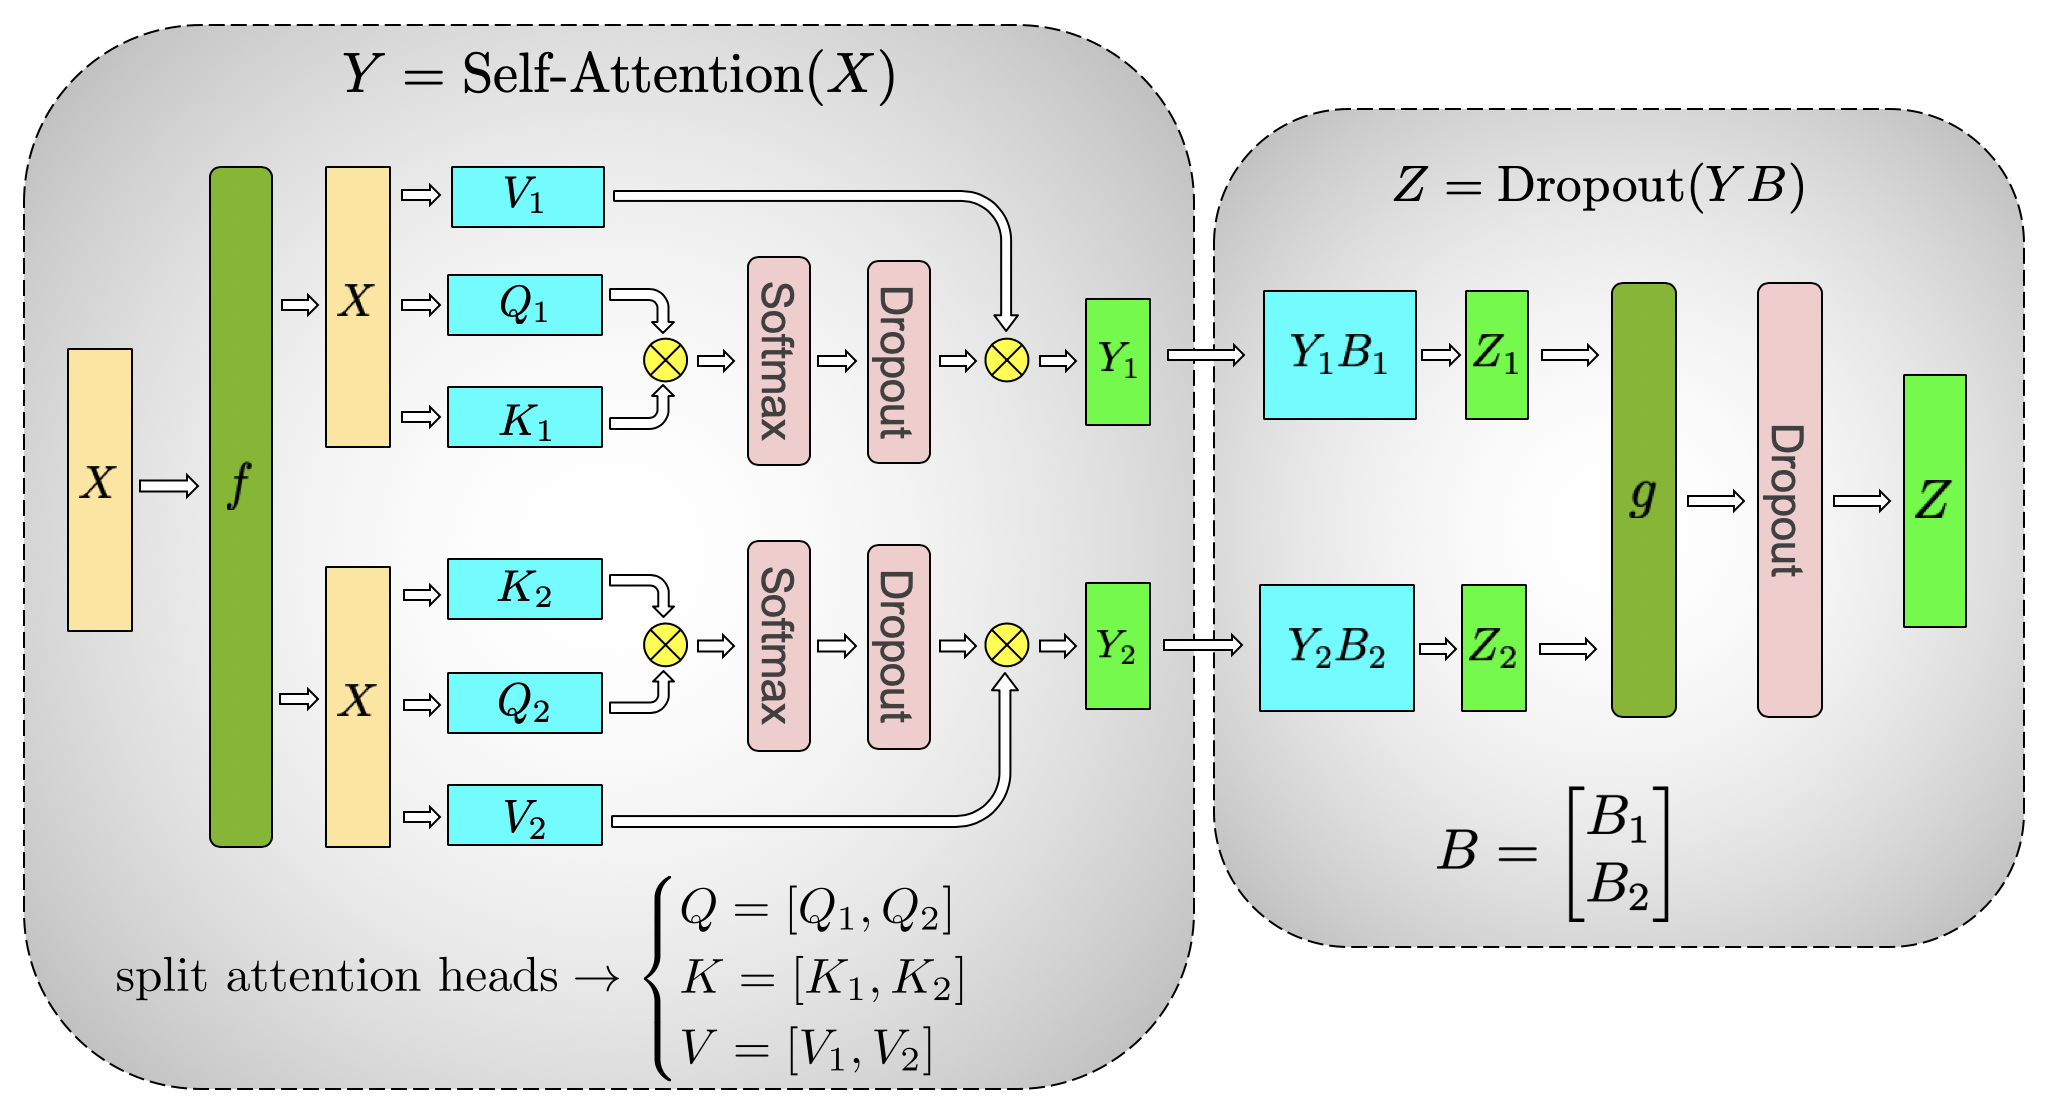
\includegraphics[scale=.45]{figures/attention_mp_2.png}
	\caption{Tensor parallelism for the \pyinline{CausalAttention} layers. Graphic from
		\cite{shoeybi2020megatronlm}. The $ f/g $ operators play the same role as in
		Fig.~\ref{fig_mlp_tensor_parallel}.}
	\label{fig_attn_tensor_parallel}
\end{figure}

\paragraph{Embedding and LM Head} Last, we can apply tensor parallelism to the language model head,
which will also necessitate sharding the embedding layer, if the two share weights, as typical.

For the LM head, we shard the output dimension as should be now familiar, ending up with $ T $
different \pyinline{(B, S, V/T)}-shaped tensors, one per group member. Rather than communicating
these large tensors around and then computing the cross-entropy loss, it is more efficient to have
each worker compute their own loss where possible and then communicate the scalar losses
around\footnote{In more detail, given the gold-answers $ y _{ bs } $ for the next-token-targets, a
	given worker can compute their contribution to the loss whenever their \pyinline{(B, S, V/T)}-shaped
	output $ z _{ bsv' } $ contains the vocabulary dimension $ v _{ * } $ specified by $ y _{ bs } $,
	otherwise those tensor components are ignored.}.

For a weight-tied embedding layer, the former construction requires \pyinline{AllReduce} in order
for every worker to get the full continuous representation of the input.

\paragraph{LayerNorm and Dropout} \pyinline{LayerNorm} instances are not sharded in pure tensor
parallelism both because there is less gain in sharding them parameter-wise, but also sharding
\pyinline{LayerNorm} in particular would require additional cross-worker communication, which we
wish to reduce as much as possible. \pyinline{Dropout} layers are also not sharded in  where
possible in pure tensor parallelism, but sharding the post-attention \pyinline{Dropout} layer is
unavoidable. It is the goal of sequence parallelism is to shard these layers efficiently; see
Sec.~\ref{subsec_seq_parallelism}.



\paragraph{Effects on Memory} The per-worker memory savings come from the sharding of the weights
and the reduced activation memory from sharded intermediate representations.

The gradient and optimizer state memory cost is proportional to the number of parameters local to
each worker (later we will also consider sharding these components to reduce redundantly-held
information). The number of parameters per worker is reduced to
\begin{align}
	N _{ \rm params } & \approx  (4 + 2E) \frac{ L D ^{ 2 } }{ T }\ ,
	\label{eq_approx_params_tensor_parallel}
\end{align}
counting only the dominant contribution from weights which scale with $ L $, since every weight is
sharded. Since all non-activation contributions to training memory scale with $ N _{ {\rm params}  }
$, this is a pure $ 1/T $ improvement.

The per-layer activation memory costs \eqref{eq_att_actmem_vanilla} and
\eqref{eq_mlp_actmem_vanilla} are altered to:
\begin{align}
	M _{ \rm act  } ^\texttt{Attention} & = BS \left ( \left (p + \frac{ 4p }{ T }+1 \right )D + \left
		(\frac{ 2p+1 }{ T } \right )AS  \right ) \nn
	M _{ \rm act  } ^\texttt{MLP}       & = \left (\frac{ 2Ep }{ T }+p+1 \right )BDS\ .
	\label{eq_act_mem_attn_mlp}
\end{align}
The derivation is similar to before. Adding in the (unchanged) contributions from
\pyinline{LayerNorm} instances, the total, leading order activation memory sums to
\begin{align}
	M _{ {\rm act}  } ^{ {\rm  total}  } & \approx  2BDLS   \left ( p \left (2+ \frac{ E+2 }{ T }\right ) + 1   \right )
	+ ABLS ^{ 2 } \left ( \frac{ 2p+1 }{ T }\right ) \label{eq_act_mem_total_tensor_parallel}\ .
\end{align}
Again, the terms which did not receive the $ 1/T $ enhancement correspond to activations from
unsharded \pyinline{LayerNorm} and \pyinline{Dropout} instances and the $ 1/T $'s improvements can
be enacted by layering sequence parallelism on top (Sec.~\ref{subsec_seq_parallelism}).


\subsection{Sequence Parallelism \label{subsec_seq_parallelism}}

In \eqref{eq_act_mem_total_tensor_parallel}, not every factor is reduced by $ T $. \textbf{Sequence
	Parallelism} fixes that by noting that the remaining contributions, which essentially come from
\pyinline{Dropout} and \pyinline{LayerNorm}\footnote{Recall, though, from
	Sec.~\ref{subsubsec_layer_norm} that the parameters in \pyinline{LayerNorm} are completely redundant
	and can simply be removed without having any effect on the expressive capabilities of the
	architecture.}, can be parallelized in the sequence dimension (as can the residual connections).

The collective communications change a bit. If we shard the tensors across the sequence dimension
before the first \pyinline{LayerNorm}, then we want the following:
\begin{enumerate}
	\item The sequence dimension must be restored for the \pyinline{CausalAttention} layer
	\item The sequence should be re-split along the sequence dimension for the next \pyinline{LayerNorm} instance
	\item The sequence dimension should be restored for the \pyinline{MLP} layer \footnote{This doesn't
		      seem like a hard-requirement, but it's what is done in \cite{korthikanti2022reducing}.}
\end{enumerate}

The easiest way to achieve the above is the following.
\begin{enumerate}
	\item If the tensor parallelization degree is $ T $, we also use sequence parallelization degree $ T
	      $.
	\item The outputs of the first \pyinline{LayerNorm} are \pyinline{AllGather}-ed to form the full-dimension
	      inputs to the \pyinline{CausalAttention}  layer
	\item The tensor-parallel \pyinline{CausalAttention} layer functions much like in
	      Fig.~\ref{fig_attn_tensor_parallel} \textit{except} that we do not re-form the outputs to
	      full-dimensionality.  Instead, before the \pyinline{Dropout} layer, we \pyinline{ReduceScatter} them
	      from being hidden-sharded to sequence-sharded and pass them through the subsequent
	      \pyinline{Dropout}/\pyinline{LayerNorm} combination, similar to the first step
	\item The now-sequence-sharded tensors are reformed with another \pyinline{AllGather} to be the full-dimensionality inputs to the
	      \pyinline{MLP} layer whose final outputs are similarly \pyinline{ReduceScatter}-ed to be
	      sequence-sharded and are recombined with the residual stream
\end{enumerate}
The above allows the \pyinline{Dropout} mask and \pyinline{LayerNorm} weights to be sharded $ T
$-ways, but if we save the full inputs to the \pyinline{CausalAttention} and \pyinline{MLP}  layers
for the backwards pass, their contributions to the activation memory are not reduced (the $ p
$-dependent terms in \eqref{eq_act_mem_attn_mlp}). In \cite{korthikanti2022reducing}, they solve
this by only saving a $ 1/T $ shard of these inputs on each device during the forward pass and then
performing an extra \pyinline{AllGather} when needed during the backwards pass. Schematics can be
sen in Fig.~\ref{fig_tensor_seq_parallel} and Fig.~\ref{fig_tensor_seq_parallel_detail} below. The
activation memory is then reduced to:
\begin{align}
	M _{ {\rm act}  } ^{ {\rm  total}  } & =\frac{ 2BDLS   \left ( p(E+4) + 1   \right ) }{ T }
	+ \frac{ ABLS ^{ 2 } \left ( 2p+1\right ) }{ T }  + \Ocal \left( BSV \right) \label{eq_act_mem_total_seq_parallel}\ .
\end{align}

In more detail:
\begin{itemize}
    \item The norms are just linear operations on the $ z _{ sd }  $, $ z' _{ sd } =
{\rm Norm}\left ( z _{ sd } \right ) $, and so we split and shard cross the sequence dimension $ z
_{ sd } \longrightarrow  z _{ (tr) d }  \equiv  \bar{z}_{ \bar{t}rd }$ with the TP-index $ t $
sharded across devices.
\item The residual stream is also sharded across the sequence dimension.
\item The sharded outputs $ \bar{z}_{ \bar{t}rd } $ must be re-formed to create the
attention and MLP inputs via an \pyinline{AllGather}. There is an optimization choice here:
either the re-formed tensors can be saved for the backward pass (negating the $ 1/T $ memory
savings) or they can be re-formed via an \pyinline{AllGather}, at the cost of extra communication.
\item Both the MLP and attention layers need to produce final sums of the form $ \bar{y} _{ s
    \bar{y} e } \bar{O} _{ \bar{t} ed } $ for some intermediate $ \bar{y} $ and weight $ \bar{O} $
    sharded across the TP-dimension $ \bar{t} $. The outputs are added to the sequence-sharded residual
    stream, and so sum is optimally computed through an \pyinline{ReduceScatter} with final shape $
    \bar{z} _{ \bar{t}'rd } = z _{ (t'r)d } = z _{  sd } =\bar{y} _{ s \bar{t} e } \bar{O} _{ \bar{t}
    ed } $. This \pyinline{ReduceScatter} (along with the \pyinline{AllGather} mentioned above)
    replace the \pyinline{AllReduce}s from the tensor-parallel case and have the same overall
    communication cost.
\end{itemize}




\begin{figure}[ht]
	\centering
	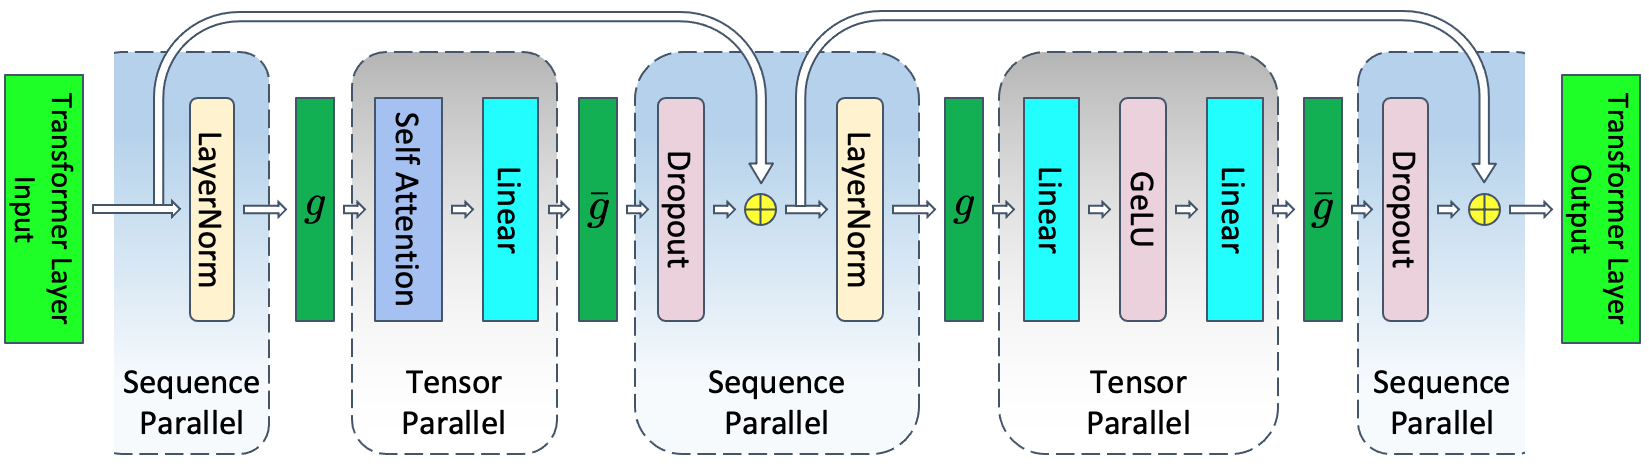
\includegraphics[scale=.25]{figures/transformer-tensor-sequence-parallel.jpg}
    \caption{Interleaved sequence and tensor parallel sections. $ g $ and $ \bar{g} $ are
    \pyinline{AllGather} and  \pyinline{ReduceScatter} in the forward pass, respectively, and swap
roles in the backwards pass. Graphic from \cite{shoeybi2020megatronlm}. }
	\label{fig_tensor_seq_parallel}
\end{figure}

\begin{figure}[ht]
	\centering
	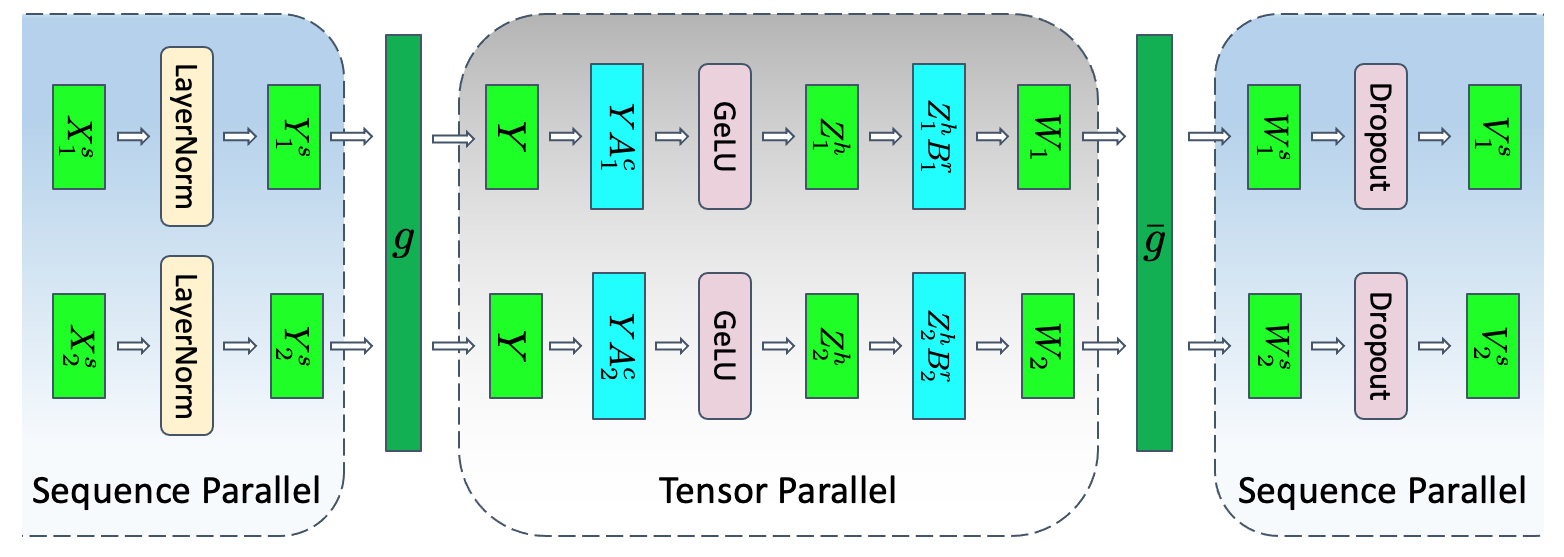
\includegraphics[scale=.25]{figures/mlp-tensor-sequence-parallel.jpg}
	\caption{Detail of the sequence-tensor parallel transition for the \pyinline{MLP} . Graphic from
		\cite{shoeybi2020megatronlm}. }
	\label{fig_tensor_seq_parallel_detail}
\end{figure}


\subsection{Pipeline Parallelism \label{subsec_pipe_parallelism}}

TODO






\subsection{Case Study: Mixed-Precision GPT3 \label{subsec_gpt_mem_study} }

Let's run through the numbers for mixed-precision GPT3 with
\href{https://bmk.sh/2020/05/29/GPT-3-A-Brief-Summary/}{parameters}:
\begin{align}
	L & = 96 \ , \quad
	D = 12288 \ ,\quad
	A = 96\ , \quad V = 50257\ .
	\label{eq_gpt_num}
\end{align}
We are leaving the sequence-length unspecified, but the block-size (maximum sequence-length) is $
	K=2048 $.


Start by assuming no parallelism at all. The total (not per-layer!) non-activation memory is
\begin{align}
	M _{ {\rm non-act}  } ^ \texttt{GPT-3} & \approx 1463\ {\rm TiB}
\end{align}
which can be broken down further as
\begin{align}
	M _{ {\rm params}  } ^ \texttt{GPT-3} & \approx 162\ {\rm TiB} \ , \quad
	M _{ {\rm grads}  } ^ \texttt{GPT-3}  \approx 325\ {\rm TiB}\ , \quad
	M _{ {\rm optim}  } ^ \texttt{GPT-3}  \approx 975\ {\rm TiB}\ .
\end{align}
The embedding matrix only makes up $ \approx .3\% $ of the total number of parameters, justifying our
neglect of its contribution in preceding expressions.


The activation memory is
\begin{align}
	M _{ {\rm act}  } ^ \texttt{GPT-3} & \approx 3 \times 10 ^{ -2 }BS\times  \left (  1  + \frac{ S
	}{ 10 ^{ 3 } } \right ) \ {\rm TiB} \ .
\end{align}
Note that the attention matrices, which are responsible for $ \Ocal \left( S ^{ 2 } \right)  $ term, will
provide the dominant contribution to activation memory in the usual $ S \gtrsim 10 ^{ 3 } $ regime.

In the limit where we process the max block size ($ S=K=2048 $), the ratio of activation to
non-activation memory is
\begin{align}
	\frac{  M _{ {\rm act}  } ^ \texttt{GPT-3}}{ M _{ {\rm non-act}  } ^ \texttt{GPT-3} }\Big| _{
	S=2048 } & \approx  .2 B \ .
\end{align}
So, the activation memory is very significant for such models.


Using tensor parallelism into the above with the maximal $ T=8 $ which can be practically used, the
savings are significant. The total memory is now
\begin{align}
	M _{ {\rm total}  } ^{ \texttt{GPT-3}  } & \approx 187\ {\rm TiB} + 10 ^{ -2 }BS + 5 \times 10 ^{
			-6} BS ^{ 2 }\ .
\end{align}




\section{Training FLOPs \label{sec_flops_training} }

The total number of floating point operations (FLOPs)\footnote{The notation surrounding
	floating-point operations is very confusing because another quantity of interest is the number
	of floating-point operations a given implementation can use \textit{per-second}. Sometimes,
	people use FLOPS or FLOP/s to indicate the rate, rather than the gross-count which has the lower
	case ``s", FLOPs, but there's little consistency in general. We will use FLOPs and FLOP/s.}  needed to process a given batch of
data is effectively determined by the number of matrix multiplies needed.

Recall that a dot-product of the form $ v \cdot M $  with $ v \in \mathbb{R}^{ m } $ and $ M \in
	\mathbb{R} ^{ m, n }$ requires $ \left (2 m-1 \right )\times n \approx 2mn$ FLOPs .
For large language models, $ m,n \sim \Ocal \left( 10 ^{ 3 } \right)  $, meaning that even expensive
element-wise operations like \pyinline{GeLU} acting on the same vector $ v $ pale in comparison by
FLOPs count \footnote{Since their FLOPs counts only scales as $ \sim \Ocal \left( n\right )  $ where
	the omitted constant may be relatively large, but still negligible when all dimensions are big.}. It
is then a straightforward exercise in counting to estimate the FLOPs for a given architecture. The
input tensor is of shape \pyinline{(B, S, D)} throughout.

\begin{nicebox}{Essentials}
	The number of FLOPs to push a batch of $ B $ of sequence-length $ S $ examples through the forwards-pass
	of a decoder-only transformer is approximately $ 2BS N _{ {\rm params}  } $ where the number of
	parameters accounts for any reductions due to tensor- and sequence-parallelism\footnote{A quick argument: a
	computation of the form $T _{ a _{ 0 }\ldots  a _{ n }j } =V _{ a _{ 0 }\ldots a _{ A
			}i }M _{ ij } $ requires $ 2A _{ 0 }\ldots A _{ n }IJ $ FLOPs where the capital letters
	represent the size of their similarly-index dimensions. Thus, the FLOPs
	essentially count the size of the matrix $ M $ (that is, $ IJ $), up to a factor of 2 times all of the
	dimensions in $ V $ which weren't summed over. Therefore, passing a
	\pyinline{(B, S, D)}-shaped tensor through the Transformer architecture would give $ \sim 2BS\times
	$(sum of sizes of all weight-matrices) FLOPs, and that this last factor is also approximately the number of
	parameters in the model (since that count is dominated by weights). Thus, FLOPs $ \approx 2BSN _{
				{\rm params}  } $. This is the correct as long as the self-attention FLOPs with $ \Ocal \left( S ^{ 2 } \right)$-dependence which we
	didn't account for here are actually negligible (true for $ S \lesssim 10  D $).}. The backwards-pass
	costs about twice as much as the forwards-pass. This is true as long as $ S \lesssim D $).
\end{nicebox}



\subsection{No Recomputation}

Start with the case where there is no recomputation activations.  These are the \textbf{model FLOPs} of
\cite{korthikanti2022reducing}, as compared to the \textbf{hardware FLOPs} which account for gradient
checkpointing.


\paragraph{\pyinline{CausalAttention}: Forwards }

The FLOPs costs:
\begin{itemize}
	\item  Generating the query, key, and value vectors: $ 6BSD ^{ 2 } $
	\item Attention scores:  $2BDS ^{ 2 }$
	\item Re-weighting values:  $2BDS ^{ 2 }$
	\item Final projection: $ 2BSD ^{ 2 } $
\end{itemize}

\paragraph{\pyinline{MLP}: Forwards}
Passing a  through the \pyinline{MLP} layer, the FLOPs due to the
first and second matrix-multiplies are equal, with total matrix-multiply FLOPs  $ 4BSED ^{ 2 } $.

\paragraph{Backwards Pass: Approximate}


The usual rule of thumb is to estimate the backwards pass as costing twice the flops as the forwards
pass. This estimate comes from just counting the number of $ \Ocal \left( n ^{ 2 } \right)$
matrix-multiply-like operations and seeing that for every one matrix multiplication that was needed
in the forward pass, we have roughly twice as many similar operations in the backwards pass.


The argument: consider a typical sub-computation in a neural network which is of the form $ z' =
	\phi \left ( W \cdot z \right ) $ where $ z', a $ are intermediate representations $ z, z' $, $ \phi
$ is some non-linearity, and where the matrix multiply inside the activation function dominates the
forwards-pass FLOPs count, as above.  Then, in the backwards pass for this sub-computation, imagine
we are handed the upstream derivative $ \partial _{ z '  } \Lcal $. In order to complete
backpropagation, we need both to compute $ \partial  _{ W }\Lcal  $ to update $ W $ and also $
	\partial  _{ z } \Lcal  $ to continue backpropagation to the next layer down. Each of these operations
will cost about as many FLOPs as the forwards-pass, hence the estimated factor of two (but, as
we will see, this is a very rough estimate).

Being more precise, let $ z $ be \pyinline{(D0, ... , Dn, J)}-shaped and let $ W $ be
\pyinline{(I, J)}-shaped such that it acts on the last index of $ z $, making $ z' $
\pyinline{(D0, ... , Dn, I)}-shaped. Denoting $D=\prod _{ i } D _{ i } $ be the number of elements
along the $ D _{ i } $ directions for brevity, the forward-FLOPs cost of the sub-computation is
therefore $ 2DIJ$.


Adding indices, the two derivatives we need are
\begin{align}
    \frac{ \partial \Lcal  }{ \partial W _{ ij } } & = \frac{ \partial \Lcal  }{ \partial z '_{ d _{ 0 } \ldots  d _{ n }i } }\phi' \left (\left (  W \cdot z \right ) _{  d _{ 0 }\ldots d _{ n }i } \right )
	z _{ d _{ 0 }\ldots  d _{ n } j } \nn
	\frac{  \partial \Lcal  }{\partial  z _{ d _{ 0 }\ldots d _{ n }j } } & = \frac{ \partial \Lcal
	}{ \partial z '_{ d _{ 0 } \ldots  d _{ n }i } }\phi' \left (\left (  W \cdot z \right ) _{  d _{
			0 }\ldots d _{ n }i } \right ) W _{ ij }\ ,\label{eq_backprop_derivatives}
\end{align}
which have shapes \pyinline{(I, J)} and \pyinline{(D0, ..., Dn, J)}, respectively. On the right
side, $ z $ and $ W \cdot  z $ are cached and the element-wise computation of $ \phi' \left ( W
\cdot z \right ) $ has negligible FLOPs count, as discussed above: its contribution is $ \Ocal
\left( 1/I \right)  $ suppressed relative to the matrix-multiplies. The FLOPs count is instead
dominated by the broadcast-multiplies, sums, and matrix-products.

The two derivatives in \eqref{eq_backprop_derivatives} each have the same first two factors in
common, and it takes $ DI $ FLOPs to multiply out these two \pyinline{(D0, ... , Dn, J)}-shaped
tensors into another result with the same shape. This contribution is again $ \Ocal \left( 1/I
\right)  $ suppressed and hence negligible. Multiplying this factor with either $ z
_{ d _{ 0 } \ldots d _{ n }i } $ or $ W _{ ij } $ and summing over the appropriate indices requires
$ 2DIJ $ FLOPs for either operation, bringing the total FLOPs to $ 4DIJ$, which is double the FLOPs
for this same sub-computation in the forward-direction, hence the rough rule of thumb\footnote{Note
    also that the very first layer does not need to perform the second term in
    \eqref{eq_backprop_derivatives}, since we do not need to backpropagate to the inputs, so the
    total backwards flops is more precisely $ 4DIJ(L-1) + 2DIJ$.}.


\paragraph{Backwards Pass: More Precise} \textbf{TODO}

\paragraph{Total Model FLOPs}


The grand sum is then\footnote{With a large vocabulary, the cost of the final language model head
	matrix multiply can also be significant, but we have omitted its $ L $-independent,  $ 2BDSV $
	contribution here. }:
\begin{align}
	C  ^{ {\rm  model}  } & \approx 12 BDLS \left ( S + \left ( 2+E \right )D \right ) \label{eq_model_flops}\ .
\end{align}
We can also phrase the FLOPs in terms of the number of parameters \eqref{eq_approx_params_tensor_parallel} as
\begin{align}
	C  ^{ {\rm  model}  } \big| _{ T=1 } & = 6BS N _{ {\rm  params}  }\times \left ( 1 + \Ocal \left( S/D\right)  \right )
\end{align}
where we took the $ T=1, D \gg S $ limit for simplicity and we note that $ BS $  is the number of
total tokens in the processed batches.


\section{Training Time \label{sec_train_time} }



Training is generally compute bound (see App.~\ref{app_compute_mem_bound}) and based on the results
of Sec.~\ref{sec_flops_training} the quickest one could possibly push a batch of data through the
model is
\begin{align}
	t _{ {\rm  min} } & = \frac{ C  ^{ {\rm  model}  }  }{   \lambda _{ {\rm FLOP/s} } }\ . \label{eq_tmin_model}
\end{align}
Expanding to the entire training run, then with perfect utilization training will take a time
\begin{align}
	t _{ {\rm  total} } & \approx  \frac{6N _{ {\rm params} } N _{ {\rm tokens} }}{   \lambda _{ {\rm FLOP/s} } }\ . \label{eq_training_rule_of_thumb}
\end{align}
Adjust $ \lambda _{ {\rm FLOP/s} } $ to the actual achievable FLOP/s in your setup to get a realistic estimate.

How many tokens should a model of size $ N _{ {\rm params} } $? Scaling laws (Sec.~\ref{sec_scaling_laws}) provide
the best known answer, and the Summer 2023 best-guess is that we optimally have $ N _{ {\rm tokens} }\approx 20 N _{ {\rm params} } $.
So that the above is
\begin{align}
	t _{ {\rm  total} } & \approx  \frac{120N _{ {\rm params} } ^{ 2 }}{   \lambda _{ {\rm FLOP/s} } }\ ,
\end{align}
leading to quadratic growth in training time.


Note that the above is only correct if we are actually only spending $C  ^{ {\rm  model}  }$
compute per iteration. This is not correct if we use gradient checkpointing and recomputation, in which case
we alternatively spend true compute  $C  ^{ {\rm  hardware}  } > C  ^{ {\rm  model}  } $,
a distinction between \textbf{hardware FLOPs} and \textbf{model FLOPs}. Two corresponding efficiency
measures are \textbf{model FLOPs utilization} (MFU) and \textbf{hardware FLOPs utilization}  (HFU).
If our iterations take actual time $ t _{ {\rm iter} } $, then these are given by
\begin{align}
	{\rm MFU} & = \frac{ t _{ {\rm iter} } }{ t _{ {\rm  min} } ^{ {\rm  model} } } \ , \quad {\rm HFU} = \frac{ t _{ {\rm iter} } }{ t _{ {\rm  min} } ^{ {\rm  hardware} } } \ , \label{eq_mfu}
\end{align}
where $ t _{ {\rm min} } ^{ {\rm  model} } $ is \eqref{eq_tmin_model} and $ t _{ {\rm min} } ^{ {\rm  hardware} } $ is similar but using
$ C  ^{ {\rm  hardware} } $.


\section{Scaling Laws \label{sec_scaling_laws}}


Empirically-discovered scaling laws have driven the race towards larger and larger models.
\begin{nicebox}{Essentials}
	Decoder-only model performance improves predictably as a function of the model size, dataset size,
	and the total amount of compute. As of Summer 2023, there is little sign of hitting any kind of wall
	with respect to such scaling improvements.
\end{nicebox}


The central parameters are:
\begin{itemize}
	\item The number of non-embedding model parameters, as excising embedding params was found to
	      generate cleaner scaling laws. Because our $ N _{ {\rm params} }$ has already been typically
	      neglecting these parameters, we will just use this symbol in scaling laws and keep the above
	      understanding implicit.\footnote{Presumably, the scaling laws are
		      cleaner with these neglected because these params do not contribute directly to
		      FLOPs, unlike most other parameters.} \cite{kaplan2020scaling}.
	\item $ C $: total compute, often in units like PFLOP/s-days $ \sim 10 ^{ 20 } $ FLOPs
	\item $ N _{ {\rm tokens} } $: dataset-size in tokens
	\item $\Lcal$: cross-entropy loss in nats
\end{itemize}
The specific form of any given scaling law should also be understood to apply to a pretty narrowly
defined training procedure, in which choices like the optimizer, learning-rate scheduler,
hyperparameter search budget, vocabulary size, tokenization, etc. are often rigidly set. Changing
different components of the training procedure is liable to create different scaling laws (though
nice laws of some form are still expected to exist).


\subsection{Original Scaling Laws}


The first scaling-laws were reported in \cite{kaplan2020scaling}.   Their simplest form relates the
value of the cross-entropy loss \textit{at convergence} (and in nats), $ \Lcal  $,  to the number of non-embedding
parameter, dataset size in token, and the amount of compute, \textit{in the limit} where only one of
this factors is bottlenecking the model\footnote{Unclear to me how you know when this is the case?}. The laws (in our notation):
\begin{itemize}
	\item $ \Lcal (N _{ {\rm params} }) \approx  \left ( N _{ {\rm  params} }^{ \star } / N _{ {\rm  params}
		      } \right ) ^{ \alpha _{ N } } $, with $ \alpha _{ N } \approx 0.076 $ and $ N _{ {\rm params} } ^{ \star }  \approx
		      8.8\times 10 ^{ 13 }$
	\item $ \Lcal (N _{ {\rm  tokens} }) \approx  \left ( N _{ {\rm tokens}} ^{ \star } / N _{ {\rm  tokens}
		      } \right ) ^{ \alpha _{ T } } $, with $ \alpha _{ T } \approx 0.095 $ and $ N _{{\rm  tokens}  } ^{  \star }  \approx
		      5.4\times 10 ^{ 13 }$
	\item $ \Lcal (C) \approx  \left ( C ^{ \star } /  C
		      \right ) ^{ \alpha _{ C } } $, with $ \alpha _{ C } \approx 0.050  $ and $ C ^{  \star }  \approx
		      3.1\times 10 ^{8} $ PFLOP/s-days, where the batch size was assumed to be chosen to be compute optimal per the criteria they outline
\end{itemize}

\begin{figure}[ht]
	\centering
	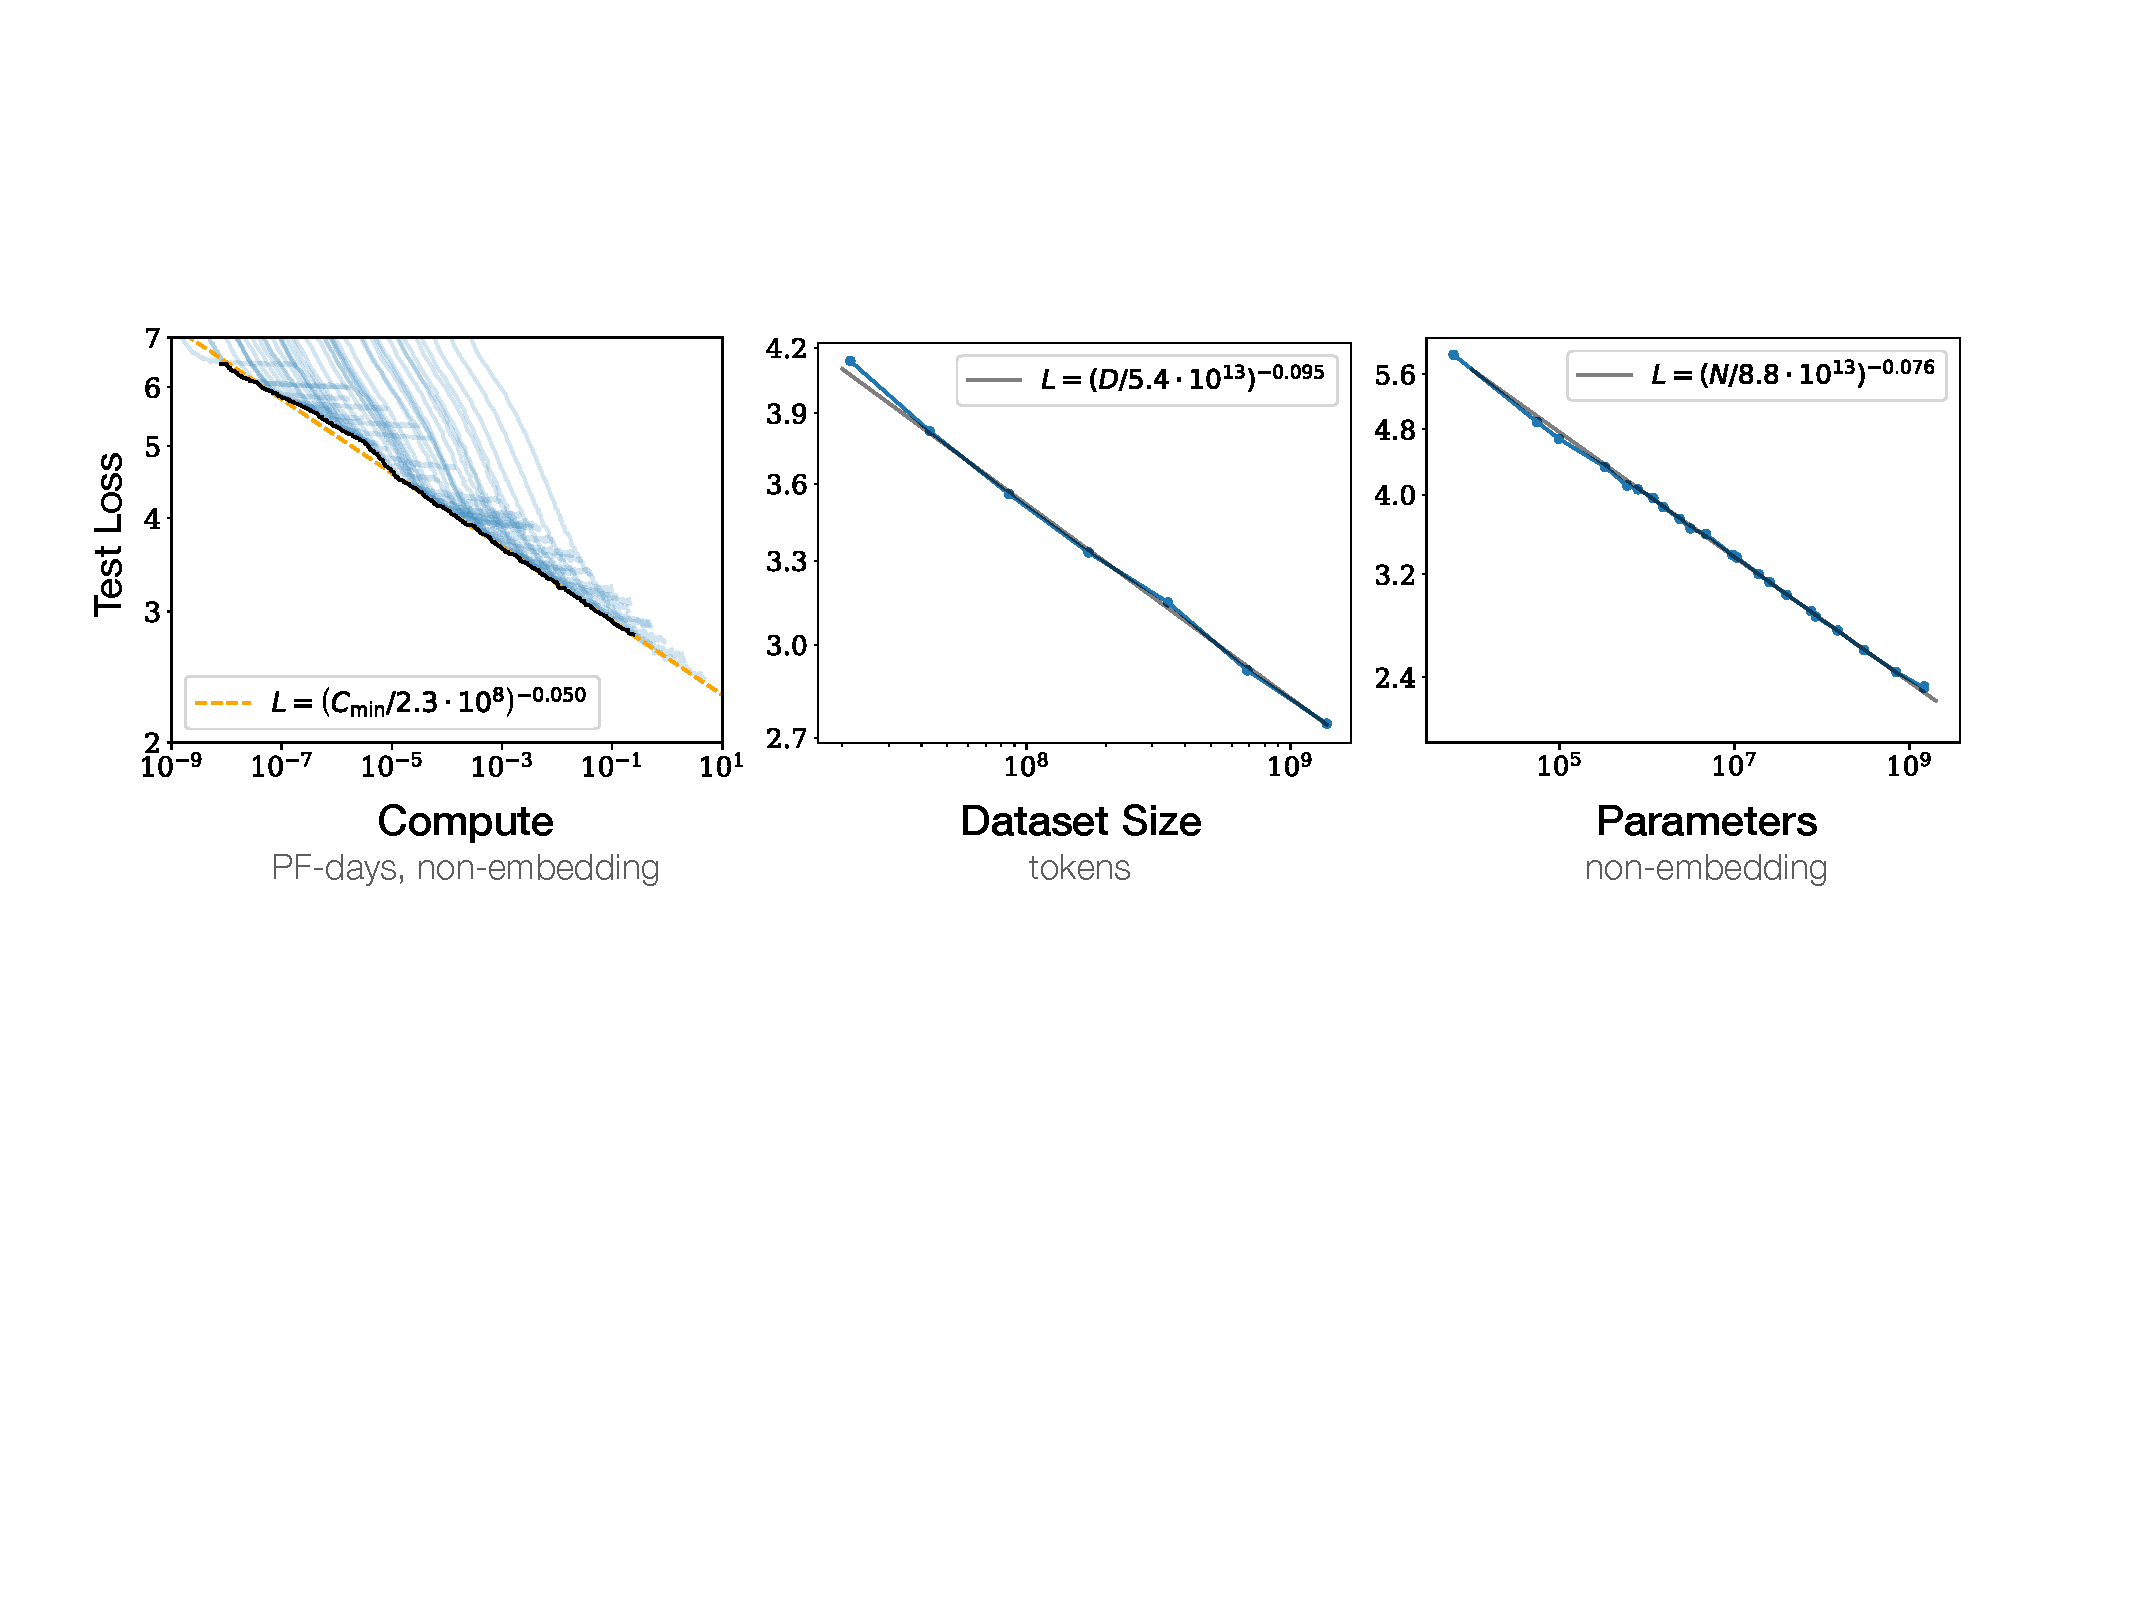
\includegraphics[scale=.5]{figures/SimplePowerLaws.pdf}
	\caption{Original scaling laws from \cite{kaplan2020scaling}.}
	\label{fig_scaling_laws_original_1}
\end{figure}


\begin{figure}[ht]
	\centering
	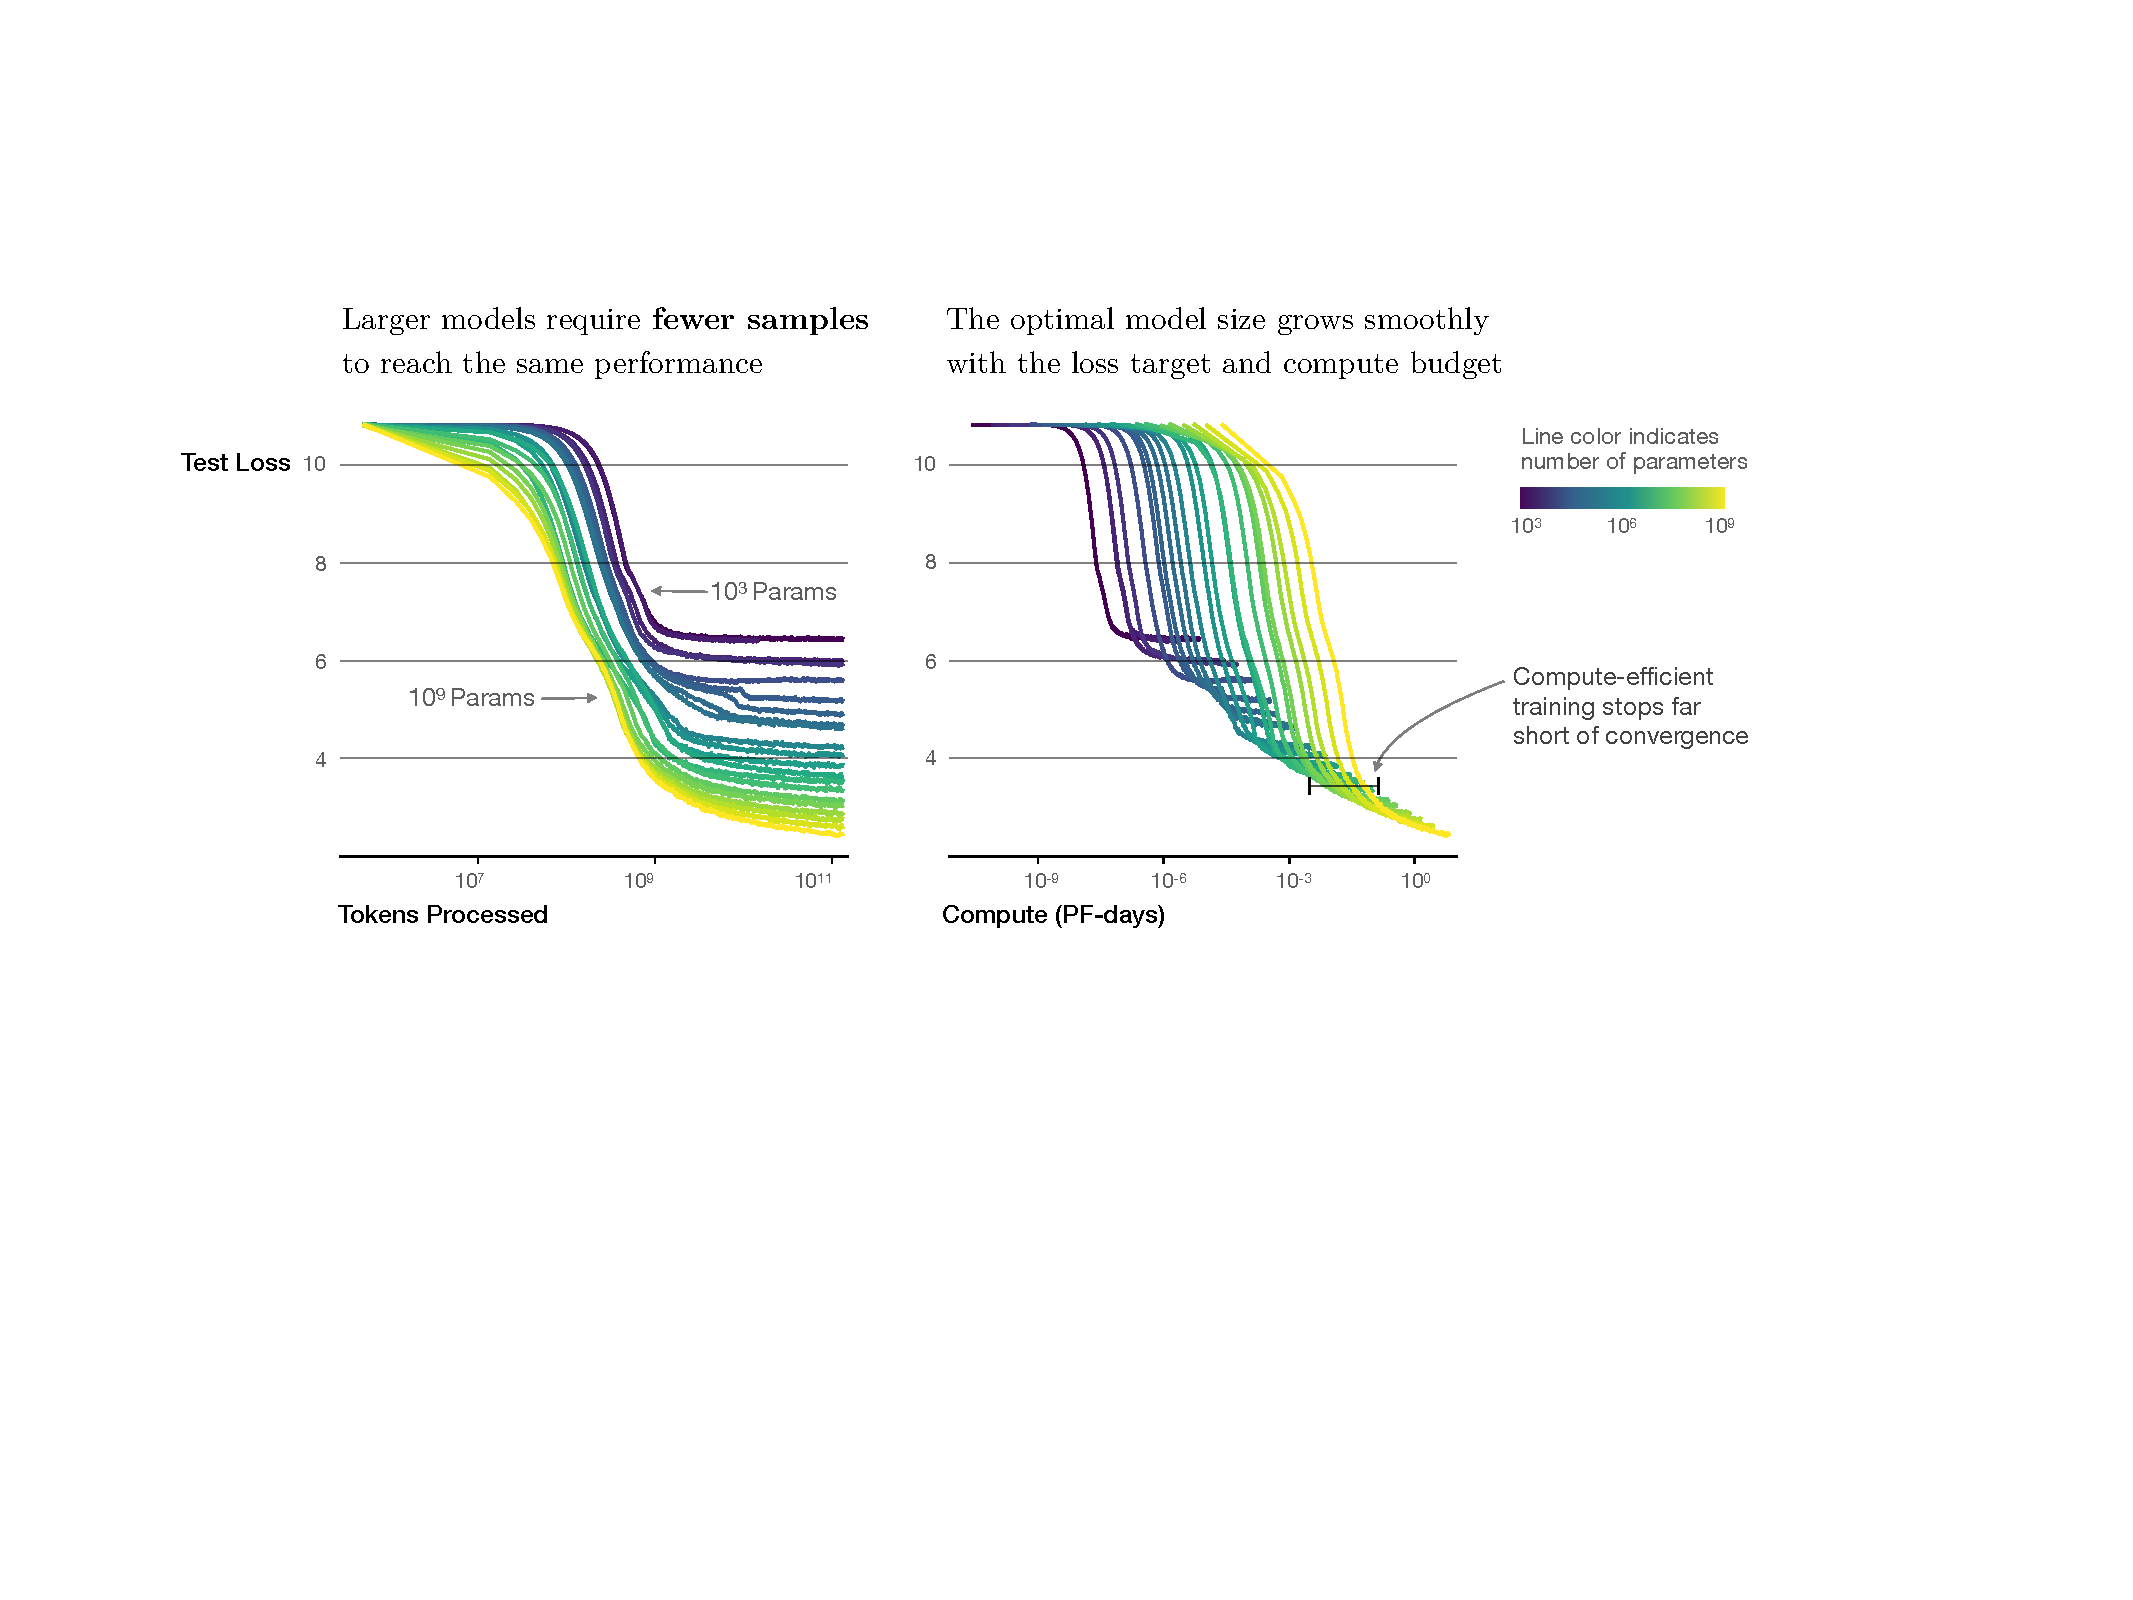
\includegraphics[scale=.5]{figures/EfficiencyIllustration.pdf}
	\caption{From \cite{kaplan2020scaling}. Larger models are much more sample-efficient (faster).}
	\label{fig_scaling_laws_original_2}
\end{figure}


\subsection{Chinchilla Scaling Laws}

As of Summer 2023, the Chinchilla scaling laws in \cite{hoffmann2022training} are the de facto best
scaling laws for guiding training. The central difference between \cite{hoffmann2022training} and
\cite{kaplan2020scaling} is that in the former they adjust their cosine learning-rate schedule to
reflect the amount of planned training, while in the latter they do not\footnote{The learning-rate
	schedule consist of a linear warm-up stage from a very small $ \eta  $ up to the largest value $ \eta _{ {\rm max} } $, after
	which the cosine bit kicks in: $ \eta (s)= \eta _{ {\rm min} } + \left ( \eta _{ {\rm max} } - \eta  _{ {\rm
				min} } \right ) \times \cos \left (\frac{ \pi s }{ 2 s _{ {\rm max} } }  \right) $ with $ s $ the
	step number. In Fig.~A1 of \cite{hoffmann2022training} they demonstrate that having the planned $ s
			_{ {\rm max} } $ duration of the scheduler be longer than the actual number of training steps is
	detrimental to training (they do not study the opposite regime), which is effectively what was done
	in \cite{kaplan2020scaling}. Probably the more important general point is again that the precise
	form of these scaling laws depend on details of fairly arbitrary training procedure choices, such as
	the choice of learning-rate scheduler.}.

Several different analyses are performed which all give very similar results. The outputs are the optimal values of $ N _{ {\rm params} }, N _{ {\rm tokens} } $ given a compute budget $ C $.
\begin{itemize}
	\item They fix various buckets of model sizes and train for varying lengths. In their resulting
	      loss-vs-FLOPs plot, they determine the model size which led to the best loss at each given FLOPs value, thereby generating
	      and optimal model size vs compute relation.
	\item They fix various buckets of FLOPs budget and train models of different sizes with that budget,
	      finding the optimal model size in each case. A line can then be fit to the optimal settings across
	      FLOPs budgets in both the parameter-compute and tokens-compute planes.
	\item  They perform a parametric fit to the loss\footnote{In \cite{hoffmann2022training} they model
		      the scaling of the test loss, while in \cite{kaplan2020scaling} they use the training loss.}:
	      \begin{align}
		      \Lcal (N _{ {\rm params} }, N _{ {\rm tokens} }) & =E + \frac{ A }{ N _{ {\rm  params} } ^{ \alpha  } }  + \frac{ B }{ N _{ {\rm tokens} } ^{ \beta  } } \label{eq_chinchilla} \ ,
	      \end{align}
	      fit over a large range of parameter and token choices. The best-fit values are:
	      \begin{align}
		      E & = 1.69 \ , \quad A = 406.4 \ , \quad B = 410.7 \ , \quad  \alpha = 0.34 \ , \quad \beta =0.28 \ .
	      \end{align}
	      Using $ C \approx 6 N _{ {\rm params}} N _{ {\rm tokens} } $, the above can be minimized at fixed compute
	      either for number of parameter or the size of the dataset.
\end{itemize}
In all cases, the findings are that at optimality  $ N _{ {\rm params} }  \sim N _{ {\rm tokens}
		}\sim C ^{ .5 } $: both the parameter and tokens budget should be scaled in equal measure.







\part{Inference}


\section{Basics and Problems}


The essentials of decoder-only inference is that a given input sequence $ x _{ bs } $ is turned into
a probability distribution $ p _{ bsv } $ over the vocabulary for what the next token might be.  Text
is then generated by sampling from $ p _{ bsv } $ in some way, appending that value to $ x _{ bs } $
to create a one-token-longer sequence, and then repeating until desired.

There are various problems that naive implementations of the above face:
\begin{itemize}
	\item Repeated computation from processing the same tokens in the same order repeatedly, at least for
	      some sub-slice of $ x _{ bs } $.
	\item Inherently sequential computation, rather than parallel
	\item Sub-optimal sampling strategies. Just choosing the most-probably token at each new step, does
	      not guarantee the most-probable overall sequence, for instance.
\end{itemize}



\section{Generation Strategies \label{sec_generation_strats} }

A quick tour of generation strategies. A very readable blog post comparing strategies can be
\href{https://huggingface.co/blog/how-to-generate}{found here.}


\subsection{Greedy \label{subsec_greedy_gen}}

The most obvious generation strategy is to take the final, \pyinline{(B, S, V)}-shaped outputs $ z
		_{ bsv } $ and just take the next token to be the most-probable one (for the final position in the
sequence): \pyinline{next_token = z[:, -1].argmax(dim=-1)}. A very minimal \pyinline{generate} method
is as below:
\pyfile[firstline=6, lastline=23]{python/greedy_generate.py}

There are various important, practical considerations which are ignored in the above implementation, including:
\begin{itemize}
	\item Since we are taking the prediction from the last (\pyinline{-1}-indexed) element in each
	      sequence, it is crucial that all padding is \textit{left}-padding, so that these final
	      elements are meaningful.
	\item Models will signal the end of generation by outputting tokenizer-specific codes, and
	      generation must respect these.
\end{itemize}
See
\href{https://github.com/huggingface/transformers/blob/04ab5605fbb4ef207b10bf2772d88c53fc242e83/src/transformers/generation/utils.py#L1115}{the
	\texttt{generate} method from the \texttt{transformers} library} for more fully-featured code
(which, correspondingly, is not always easy to follow).

\subsection{Simple Sampling: Temperature, Top-$ k $, and Top-$ p $ \label{subsec_simple_sampling}}

The next-most-obvious strategy is to choose the next token by drawing from the probability
distribution defined by the $ z _{ bsv } $. There are various refinements of this idea.

A one-parameter generalization of this strategy
introduces a (physics-motivated) \textbf{Temperature} which just adjusts the scale of the logits:
\begin{py}
	next_token = torch.multinomial((z[:, -1] / temp).softmax(dim=-1), num_samples=1)
\end{py}
assuming \pyinline{z} are the final logits. Larger temperature yields a larger variance in the chosen
tokens.

With temperature sampling, there is still a non-zero chance of choosing an extremely improbable token,
which is undesirable if you do not trust the tails of the distribution. Two common truncation
strategies which guard against this:
\begin{itemize}
	\item \textbf{Top-}$ k $: Only choose from the top-$ k $ most-probable examples (re-normalizing
	      the probabilities across those $ k $ samples)
	\item \textbf{Top-}$  p$: Only choose from the top-however-many most-probable examples whose
	      probabilities sum to $ p $ (again re-normalizing probabilities). This is also sometimes called
	      \textbf{nucleus sampling}.
\end{itemize}


\subsection{Beam Search \label{subsec_beam_search}}

Choosing, say, the most-probable next-token at each step is not guaranteed to yield the most
probable \textit{sequence} of tokens. So, \textbf{Beam Search} explores multiple sequences, using
different branching strategies, and the probabilities of the various beam sequences can be compared
at the end. Important note: generating the most-probable text is not necessarily equal to the most
human-like text \cite{holtzman2020curious}.





\section{The Bare Minimum and the kv-Cache \label{sec_kv_cache}}


There are two separate stages during generation. First, an original, to-be-continued series of prompts
$ x _{ bs }  $ can be processed in parallel to both generate the first prediction and populate any
intermediate values we may want to cache for later. We follow \cite{pope2022efficiently} and call this the
\textbf{prefill} stage. For this procedure, we require the entire $ x _{ bs } $ tensor.

In the second, iterative part of generation (the \textbf{decode} stage) we have now appended
one-or-more tokens to the sequence and we again want the next prediction, i.e. \pyinline{z[:, -1, :]}
for the last-layer outputs $ z _{ bsd } $. In this stage, we can avoid re-processing the entire $ x
		_{ bs } $ tensor and get away with only processing the final, newly added token, \textit{if} we are
clever and cache old results (and accept a very reasonable approximation).

The important pieces occur in the \pyinline{CausalAttention} layer, as that's the only location in
which the sequence index is not completely parallelized across operations. Referring back to
Sec.~\ref{subsubsec_attn_layer}, given the input $ z _{ bsd } $ of the \pyinline{CausalAttention}
layer, the re-weighted value vectors\footnote{Summed over $ s' $, but concatenating the different $
		a $ values over the $ f $ dimension.} $ w ^{ a }_{ bss'd } v ^{ a } _{ bs'f } $ are the key objects
which determine the next-token-prediction, which only depends on the $ s=-1 $ index values.
Therefore, we can cut out many steps and the minimum requirements are:
\begin{itemize}
	\item Only the attention weights $ w ^{ a }_{ bss'd }$ with $ s=-1 $ are needed
	\item The only query values $ q ^{ a }_{ bsd } $ needed to get the above are those with $ s=-1 $
	\item Every component of the key and value vectors $k ^{ a }_{ bsd }, v ^{ a }_{ bsd } $ is
          needed, but because of the causal mask, all components except for the last in the sequence
          dimension ($ s\neq -1 $) are the same as they were in the last iteration, up to a shift by
          one position\footnote{This is where we need to accept a mild approximation, if using a
              sliding attention window. With an infinite context window, if we add a label $ t $
              which indexes the iteration of generation we are on, then we would have that $ z ^{
              (t+1) } _{ bsd } = z ^{ (t)} _{ b (s-1)d } $ for every tensor in the network, except
              for when $ s=-1 $, the last position. The finiteness of the context window makes this
              statement slightly inaccurate because we can only ever keep $ K $ positions in context
              and the loss of the early tokens upon sliding the window over will slightly change the
          values in the residual stream.}
\end{itemize}

So, we are led to the concept of the \textbf{kv-cache} in which we cache old key and query vectors for generation.
The cache represents a tradeoff: fewer FLOPs are needed for inference, but the memory costs are potentially
enormous, since the size of the cache grows with batch size and sequence length:
\begin{align}
	M _{ {\rm kv-cache}  } & = 2pBDLS /T\ ,  \label{eq_kv_cache_memory}
\end{align}
in the general case with tensor-parallelism. This can easily be larger than the memory costs of the
model parameter: $ M _{ {\rm params}  } ^{ {\rm  inference}  } \sim p N _{ {\rm params}  } \sim p LD
^{ 2 }  $ (dropping $ \Ocal \left( 1 \right)  $ factors), so that the cache takes up more memory
when $ BS \gtrsim D $, i.e. when the total number of token exceeds the hidden dimension. Using the
kv-cache eliminates a would-be $ \Ocal \left( S ^{ 2 } \right)  $ factor in the FLOPs needed to
compute a new token, reducing it to linear-in-$ S $ dependence everywhere.


A very minimal implementation\footnote{Warning: very non-optimized code! Purely pedagogical.} is below:
\pyfile[firstline=6, lastline=37]{python/causal_attention_kv_cache.py}


\section{Basic Memory, FLOPs, Communication, and Latency}

The essentials of inference-time math, much of it based on \cite{kipply_inference_math}.

\paragraph{Naive Inference} Processing a single \pyinline{(B, S, D)}-shaped tensor to generate a
single next input costs the $ 2BSN _{ {\rm params}  } $ FLOPs we found for the forwards-pass in
Sec.~\ref{sec_flops_training} (assuming $ S \lessim D $). Memory costs just come from the parameters
themselves: $ M _{ {\rm infer}  }^{ {\rm naive}  }=pN _{ {\rm params}  } $. Per the analysis of
App.~\ref{app_compute_mem_bound}, naive inference is generally compute-bound and so the
per-token-latency is approximately\footnote{Assuming we do the naive thing here and generate the
    next token in a similarly naive way, shifting over the context window.}  $  2BSN _{ {\rm params}
    }/ \lambda _{ {\rm FLOP/s}  } $ where the FLOPs bandwidth in the denominator is again defined in
    App.~\ref{app_compute_mem_bound}.

\paragraph{kv-Cache Inference}
The FLOPs requirements for the hidden-dimension matrix multiplies during generation are $2BN _{ {\rm params}  } $,
since we are only processing a single token, per previous results.   This is in addition to the up-front cost of $ 2BSN _{
			{\rm params}} $ for the prefill. But, the memory requirements are raised to
\begin{align}
	M _{ {\rm infer}  }^{ {\rm kv-cache}  } & =pN _{ {\rm params}  } + 2pBDLS/T\ .
\end{align}
Inference now has a computational-intensity of
\begin{align}
	\frac{ C _{ {\rm infer} } ^{ {\rm kv-cache} } }{ M _{ {\rm infer}  }^{ {\rm kv-cache}  } } & \sim \frac{ BD }{ S } \ ,
\end{align}
dropping $ \Ocal \left( 1 \right)  $ factors, is now memory-bound (again, see
App.~\ref{app_compute_mem_bound}), and has per-token-latency of approximately $ M _{ {\rm infer} }/
	\lambda _{ {\rm mem} }$, unless the batch-size is very large.


\paragraph{Intra-Node Communication} For $ T $-way tensor parallelism, two \pyinline{AllReduce}s are
needed, one for each \pyinline{MLP} and each \pyinline{CausalAttention} layer, where each
accelerator is sending $ pBDS  $ bytes of data (see Sec.~\ref{subsec_tensor_parallelism}). This
requires a total of $ 4\left ( T-1 \right ) pBDS/T \approx 4pBDS $ bytes to be transferred between
workers in the tensor-parallel group (see Foot.~\ref{foot_all_reduce}), taking a total of $ \sim  4pBDLS/
	\lambda _{ {\rm comms} }  $ time for the model as a whole. For an A100 80GiB, \pyinline{torch.float16} setup, this is $ \sim
	BDS \times  10 ^{ -11 } \ {\rm sec} $


\paragraph{Latency} TODO



\section{Case Study: \href{https://huggingface.co/tiiuae/falcon-40b-instruct?_sm_vck=j230jZ2ssDkkPfJTfRt6tjQNTQZJ65N7VDWmj5Ff6f3jZ3mhh2Pq}{Falcon-40B}}

Let's work through the details of the kv-cache for Falcon-40B\footnote{Falcon actually uses
	multi-query attention, which changes the computations here, but we will pretend it does not in this
	section for simplicity.} with $ D=8192 $, $ L=60 $, $ S=2048 $.  In half, $ p=2 $ precision, the model weights just about fit on an
80GiB A100, but this leaves no room for the cache, so we parallelize $ T $ ways across $ T $ GPUs,
assumed to be on the same node. The total memory costs are then
\begin{align}
	M _{ {\rm  total} } & \approx  \frac{ {\rm 80GiB} + {\rm 4GiB}\times B }{ T } \ .
\end{align}
This means that in order to hit the compute-bound threshold of $ B \sim 200 $ (see
App.~\ref{app_compute_mem_bound}) we need at least $ T=4 $ way parallelism.  Taking $ T=4 $, and
running at capacity with $ B \sim 200$ so that we are compute-bound, the per-iteration latency from
computation alone is approximately $ \frac{2BN _{ {\rm params} } }{ \lambda _{ {\rm FLOP/s} } T} \sim
$13ms, i.e. we can give $ \sim $200 customers about $ \sim $75 tokens-per-second at this
rate\footnote{Average human reading speed is about $ \sim 185$ words/minute, or $ \sim 4
	$tokens/sec.}, if this were the only latency consideration.











\appendix



\section{Conventions and Notation\label{app_conventions}}


We loosely follow the conventions of \cite{korthikanti2022reducing}.  Common parameters:
\begin{itemize}
	\item $ A $: number of attention heads
	\item $ B $: microbatch size
	\item $ C $: compute (FLOPs)
	\item $ D $: the hidden dimension size
	\item $ E $: expansion factor for MLP layer (usually $ E=4 $)
	\item $ H $: $ D/A $, the head dimension size
	\item $ K $: the block size (maximum sequence length\footnote{In the absence of methods such as         ALiBi \cite{ALiBi}  can be used to extend the sequence length at inference time.})
	\item $ L $: number of transformer layers
	\item $ N _{ {\rm params}  } $: total number of model parameters
	\item $ P $: pipeline parallel size
	\item $ S $: input sequence length
	\item $ T $: tensor parallel size
	\item $ V $: vocabulary size
	\item $ t $: various timescales
	\item $ p $: the precision of the elements of a tensor in bytes
	\item $ \lambda  $: various rates, e.g. $ \lambda _{ {\rm mem}  } $ is memory bandwidth
\end{itemize}
Where it makes sense, we try to use the lower-case versions of these characters to denote the
corresponding indices on various tensors. For instance, an input tensor with the above batch size,
sequence length, and vocabulary size would be written as $ x _{ bsv } $, with $ b \in \left \{ 0,
	\ldots, B - 1 \right \} $, $ s \in \left \{ 0, \ldots, S - 1\right \} $, and $  v \in \left \{ 0,
	\ldots, V -1\right \}$ in math notation, or as \mintinline{python}{x[b, s, v]} in code.  Typical
transformers belong to the regime
\begin{gather}
	V \gg D, S \gg L, A \gg P, T \ .  \label{app_eq_transformers_approxs}
\end{gather}
For instance, GPT-2 and GPT-3 \cite{gpt2radford2019language, gpt3brown2020language} have $ V \sim
	\Ocal \left( 10 ^{ 4 } \right)  $, $ S, L \sim \Ocal \left( 10 ^{ 3 } \right)  $, $ L, A \sim \Ocal
	\left( 10 ^{ 2 } \right)  $. We will often assume also assume that\footnote{This condition ensures
	that the $ \Ocal \left( S ^{ 2 } \right)  $ FLOPs cost from self-attention is negligible
	compared to $ \Ocal \left( D ^{ 2 } \right)  $ contributions from other matrix multiplies.  It
	should be noted that in Summer 2023 we are steadily pushing into the regime where this condition
	does \textit{not}  hold.} $ S \lesssim D $ or the weaker\footnote{This condition ensures that the
	cost of reading the $ \Ocal \left( D ^{ 2 } \right)  $ weights is more than the cost of reading in
	the $ \Ocal \left( BSD \right)  $ entries of the intermediate representations.} $ BS \lesssim D $.

As indicated above,  we use zero-indexing. We also use \pyinline{python} code
throughout\footnote{Written in a style conducive to latex, e.g. no type-hints and clarity
prioritized over optimization.}  and write all ML code using standard \pyinline{torch} syntax. To
avoid needing to come up with new symbols in math expressions we will often use expressions like $ x
\leftarrow f(x) $ to refer to performing a computation on some argument ($ x $) and assigning the
result right back to the variable $ x $ again.

Physicists often joke (half-seriously) that Einstein's greatest contribution to physics was his
summation notation in which index-sums are implied by the presence of repeated indices and summation
symbols are entirely omitted. For instance, the dot product between two vectors would be written as
\begin{align}
	\vec{x} \cdot \vec{y} & = \sum _{ i } x _{ i } y _{ i } \equiv x _{ i } y _{  i }
	\label{app_eq_einstein_sum}
\end{align}
We use similar notation which is further adapted to the common element-wise deep-learning
operations.  The general rule is that if a repeated index appears on one side of an equation, but
not the other, then a sum is implied, but if the same index appears on both sides, then it's an
element-wise operation. The Hadamard-product between two matrices $ A $ and $ B $ is just
\begin{align}
	C _{ ij } & = A _{ ij } B _{ ij }\ .
\end{align}
Einstein notation also has implementations available for \pyinline{torch}:
\href{https://rockt.github.io/2018/04/30/einsum}{see this blog post on \pyinline{einsum}} or the
\href{https://einops.rocks/1-einops-basics/}{\pyinline{einops}} package.

In particular, we use \pyinline{einops} notation for concatenation and splitting: $ A _{ c } = A _{
    (de) }= B _{ de } $\footnote{The indexing is all row-major: if $ A _{ i } $ is $
        I$-dimensional, $ i \in \{0, \ldots, I-1\} $, then if we split this index as $ A _{ i } = A
        _{ (jk) } \equiv \bar{A} _{ jk } $, then the indices $ j, k $ will range over $ j \in \{0,
    \ldots , J\} $, $ k\in \{0, \ldots , K\} $ with $ I =J \times K $ and where numerically $ i = j
\times K + k $. More complex cases follow by induction.}. We will sometimes use a bar to indicate
tensors which  are derived from other tensors through such splitting operations, usually in the
context of tensor-sharding where devices only locally hold some shard of the tensor. In this
context, only some of the dimensions will be sharded across devices, and we may also put a bar over
the corresponding sharded index. For instance, consider a two-dimensional tensor $ M _{ ab } $ of
shape \pyinline{M.shape=(A, B)}: sharding this tensor across two devices across the final index
results in a tensor $ \bar{M}_{ a \bar{b} } $ which is of shape \pyinline{M_bar.shape=(A, B/2)} on
each device. As here, we will sometimes use bars to denote indices which are sharded over different
devices.

We also put explicit indices on operators such as Softmax to help clarify the relevant
dimension, e.g. we would write the softmax operation over the $ b $-index of some batched
tensor $ x _{ bvd\ldots } $ as
\begin{align}
	s _{ bvd\ldots } & = \frac{ e^{ x _{ bv d\ldots}  } }{ \sum _{ v = 0 } ^{  v= V-1 } e^{ x _{
						bvd\ldots } } } \equiv
	\Sm _{ v } \ x _{ bvd\ldots }
	\ , \label{app_eq_einstein_softmax}
\end{align}
indicating that the sum over the singled-out $ v $-index is gives unity.

\section{Collective Communications \label{app_collective_communications} }

A quick refresher on common distributed
\href{https://docs.nvidia.com/deeplearning/nccl/user-guide/docs/usage/collectives.html}{communication
    primitives}.  Consider $ N $ workers with tensor data $ x ^{ (n) }  $ of some arbitrary shape
    \pyinline{x.shape}, which takes up $ M $ bytes of memory, where $ n $ labels the worker and any
    indices on the data are suppressed. The $ n=0 $ worker is arbitrarily denoted the
    \textit{chief}.  Then, the primitive operations are:
\begin{itemize}
	\item \pyinline{Broadcast}: all workers receive  the chief's data, $ x ^{ (0) }  $.
	\item \pyinline{Gather}: all workers communicate their data $ x _{ n } $ to the chief, e.g. in a
	      concatenated array $ [x ^{ 0 }, x ^{ 1 }, \ldots , x ^{ N-1 }] $.
	\item \pyinline{Reduce}: data is \pyinline{Gather}-ed to the chief, which then performs some
	      operation (\pyinline{sum}, \pyinline{max}, \pyinline{concatenate}, etc.) producing a new tensor $
		      x' $ on the chief worker.
    \item \pyinline{ReduceScatter}: a reducing operation (e.g. \pyinline{sum}) is applied to the $ x
        ^{ (n) } $ to produce a $ x' $ of the same shape (e.g. $ x'= \sum x ^{ (n) } $) and each
        worker only receives a $ 1/N $ slice (and hence $ M/N $ byte) of the result\footnote{Note that \pyinline{AllGather}
            and \pyinline{ReduceScatter} are morally conjugate to each other. In the former, each
            worker ends up with $ N $ times as much data as they started with, while in
        \pyinline{ReduceScatter} they end up with $ 1/N $ of their initial data. One is nearly a
        time-reversed version of the other, which is a way of remembering that they have the came
        communication cost. They also compose to produce an output of the same initial size, as in
        \pyinline{AllReduce}.}. A ring implementation sends $ M \times \frac{ N-1 }{ N } $ bytes
        over each link in the ring.
    \item \pyinline{AllGather}: all data $ x ^{ (n) } $ is communicated to all workers; each worker
        ends up with the array $ [x ^{ 0 }, x ^{ 1 }, \ldots , x ^{ N-1 }] $. Functionally
        equivalent to a \pyinline{Gather} followed by \pyinline{Broadcast}. A ring implementation
        sends $ M \times \left ( N-1 \right ) $ bytes over each link in the ring.
	\item \pyinline{AllReduce}: all workers receive the same tensor $ x' $ produced by operating on
	      the $ x ^{ (n) } $ with \pyinline{sum}, \pyinline{mean}, etc. Functionally equivalent to a
	      \pyinline{Reduce} followed by \pyinline{Broadcast}, or a \pyinline{ReduceScatter} followed
	      by a \pyinline{AllGather} (the more efficient choice\footnote{The former strategy scales
		      linearly with the number of worker, while the latter strategy underlies ``ring"
		      \pyinline{AllReduce} which is (nearly) independent of the number of workers: if each
		      worker carries data of size $ D $ which is to be \pyinline{AllReduce}-d, a total of $
			      \frac{ 2 \left ( N-1 \right )D }{ N } $ elements need to be passed around.
		      \href{https://andrew.gibiansky.com/blog/machine-learning/baidu-allreduce/}{See this blog
			      post for a nice visualization} or \cite{bandwidthOptimalAllReduce2009} for a relevant
              paper.\label{foot_all_reduce}}). In the latter case, the total cost is $ 2M \times
              \frac{ N-1 }{ N } $, due to \pyinline{AllReduce}-ing the initial $ M $-sized data, and
              then \pyinline{AllGather}-ing the $ M/N $-sized reductions.
      \item  \pyinline{Scatter}: One worker gives shards of a tensor to all workers. If the worker
          is scattering tensor $ T _{ x } $ over the given index, a \pyinline{Scatter}
          effectively shards this as $ T _{ x } \longrightarrow T _{ (\bar{r}y) } $, each worker
          getting a $ \bar{r} $-shard.
      \item  \pyinline{AllToAll}: All workers receive shards of all others worker's tensors.  If
          every worker has a tensor $ T _{ \bar{r}y } $, for one value of $ \bar{r} $, which we
          imagine came from a sharding a tensor $ T _{ x } = T _{ (\bar{r}y) } $, then an
          \pyinline{AllToAll} over the $ y $ index produces produces the tensor $ T _{ z \bar{r} }$
          defined by$ T _{ z \bar{r} }= T _{ x } $ on all workers.
\end{itemize}



\section{Hardware}

Basic information about relevant hardware considerations. Much of the following is from the
\href{https://docs.nvidia.com/deeplearning/performance/dl-performance-gpu-background/index.html}{NVIDIA
	docs}.



\subsection{NVIDIA GPU Architecture}

NVIDIA GPUs consist of some amount of relatively-slow off-chip DRAM memory\footnote{This is the number usually reported when
	discussing a given GPU, e.g. 32GiB for the top-of-the-line A100}, relatively-fast on-chip SRAM, and
a number of \textbf{streaming multiprocessors} (SMs) which perform the parallel computations.  Inside
more-recent GPUs, the SMs carry both ``CUDA cores" and "Tensor cores", where the latter are used for matrix-mulitiplies
and the former for everything else.


A few numbers of primary importance:
\begin{itemize}
	\item The rate at which data can be transferred from DRAM to SRAM ($ \lambda _{ {\rm mem} } $)
	\item The number of FLOP/s, which is more fundamentally computed by multiplying the number of
	      SMs by the FLOPS/cycle of each SM for the specific operation under consideration (see the NVIDIA
	      docs) by the clock rate: $ N _{ {\rm SM} }\cdot  \lambda _{ {\rm FLOPs/cycle} }\cdot  \lambda _{
			      {\rm clock} } $
\end{itemize}

The terminology and structure of the memory hierarchy is also important to understand. Types of
memory, from slowest to fastest:
\begin{itemize}
	\item \textbf{Global} memory is the slow, but plentiful, off-chip DRAM. It is the type of memory
	      typically used as kernel arguments
	\item \textbf{Constant} memory is read only and accessible by all threads in a given block. The
	      size of arrays in constant memory must be known at compile time
	\item \textbf{Local Memory} is similarly slow to global memory, but more plentiful than register
	      memory, and privately to individual threads and is allocated from within a kernel. When
	      registers run out, local memory fills the gap
	\item \textbf{Shared} memory is shared between all threads in a given block. Shared memory is
	      effectively a user-controlled cache. The size of arrays in shared memory must  be known at
	      compile time
	\item \textbf{Registers} hold scalar values and small tensors whose values are known at compile
	      time. They are local to each thread and they are plentiful since each thread needs its own
	      set of registers: 65,536 = $ 2 ^{ 16 } $ registers per SM an A100.
\end{itemize}
\href{https://www.youtube.com/watch?v=QQceTDjA4f4&t=2124s}{An excellent video overview of CUDA and NVIDIA GPU architecture which covers some of the above is here.}

\subsection{CUDA Programming Model}

The CUDA programming model uses a hierarchy of concepts:
\begin{itemize}
    \item \textbf{Threads}  are the fundamental unit of execution\footnote{Threads are always
        physically launched in \textbf{Warps} which consist of 32 threads.} which each run the same
        CUDA \textbf{Kernel}, or function, on different data inputs in parallel. Threads within the
        same block (below) may share resources, like memory, and may communicate with each other.
        Individual threads are indexed through the \textbf{threadIdx} variable, which has
        \cudainline{threadIdx.{x, y, z}} attributes with \cudainline{threadIdx.x} in
        \cudainline{0, ..., blockDim.x -1} and similar.

	\item Threads (and hence warps) are organized into 3D \textbf{blocks}. The size and indices of
	      the blocks can be accessed through the \cudainline{blockDim} and \cudainline{blockIdx}
	      variables, respectively, with \cudainline{blockIdx.x} in \cudainline{0, ..., gridDim.x - 1}.
	      \cudainline{blockDim.x *blockDim.y * blockDim.z} total threads run in a block.
	\item Blocks are organized into 3D \textbf{groups}. The size of the gird dimensions can be
	      accessed through the \cudainline{gridDim} variable, with similar attributes to the above. \\
	      \cudainline{gridDim.x * gridDim.y * gridDim.z} total blocks run in a grid.
\end{itemize}

The number of threads which can be launched in a given block is hardware limited; A100 80GiB GPUs
can run up to 1024 threads in a SM at a time (32 blocks with 32 threads each), for instance. Hence,
block and grid sizes need to be adjusted to match the problem size. There are also important memory
access considerations here. The 1024 threads which can be launched can also read sequentially from
memory and efficient usage implies that choosing the block size such that we are doing these reads
as often as possible is ideal.

\subsection{NVIDIA GPU Stats \label{app_gpu_stats}}


Summary of some relevant NVIDIA GPU statistics:
\begin{center}
	\begin{tabular}{| c |c| c |c |c| c| }\hline
		GPU                                                                                                                                  & Memory & $ \lambda _{ {\rm FLOP/s }  } $ & $ \lambda _{ {\rm mem}  } $ & $ \lambda _{ {\rm math}  } $ & $ \lambda _{ {\rm comms}  } $ \\ \hline
		\href{https://www.nvidia.com/content/dam/en-zz/Solutions/Data-Center/a100/pdf/nvidia-a100-datasheet-nvidia-us-2188504-web.pdf}{A100} & 80GiB  & 312  TFLOP/s                    & 2.0 TiB/s                   & 156 FLOPS/B                  & 300 GiB/s                     \\ \hline
		\href{https://www.nvidia.com/content/dam/en-zz/Solutions/Data-Center/a100/pdf/nvidia-a100-datasheet.pdf}{A100}                       & 40GiB  & 312  TFLOP/s                    & 1.6 TiB/s                   & 195 FLOPS/B                  & 300 GiB/s                     \\ \hline
		\href{https://images.nvidia.com/content/technologies/volta/pdf/volta-v100-datasheet-update-us-1165301-r5.pdf}{V100}                  & 32GiB  & 130  TFLOP/s                    & 1.1 TiB/s                   & 118  FLOPS/B                 & 16 GiB/s                      \\ \hline
	\end{tabular}
\end{center}
where
\begin{itemize}
	\item $ \lambda _{ {\rm  FLOP/s}  } $ is flops bandwidth (for \pyinline{float16/bfloat16}  multiply-accumulate ops)
	\item $ \lambda _{ {\rm  mem}  } $ is memory bandwidth
	\item $ \lambda _{ {\rm  math}  } = \frac{  \lambda _{ {\rm FLOP/s}  } }{ \lambda _{ {\rm mem} } } $ is \href{https://docs.nvidia.com/deeplearning/performance/dl-performance-gpu-background/index.html#gpu-arch}{math bandwidth}
	\item $ \lambda _{ {\rm  comms}  } $ is one-way communication bandwidth
\end{itemize}
A useful approximate conversion rate is that $ 1 \ {\rm TFLOP/s} \approx 100\  {\rm PFLOP/day} $.

Important practical note: the $ \lambda _{ {\rm FLOP/s} } $ numbers should be taken as aspirational.
Out-of-the box, \pyinline{torch.float16} matrix-multiplies in \pyinline{torch} with well-chosen
dimensions tops out around $ \sim 250 $ FLOPS/s




\section{Compute-bound vs Memory-bound \label{app_compute_mem_bound} }

If your matrix-multiplies are not sufficiently large on, you are wasting resources
\cite{he2022brrrrfromfirstprinciples}. The relevant parameters which determine sufficiency are $
	\lambda _{ {\rm FLOP/s}  } $ and $ \lambda _{ {\rm mem}  } $, the FLOPs and memory bandwidth,
respectively. The ratio $  \lambda _{ {\rm math}  } \equiv \frac{  \lambda _{ {\rm FLOP/s}  } }{
		\lambda _{ {\rm mem}  } }   $ determines how many FLOPS you must perform for each byte loaded from
memory; see App.~\ref{app_gpu_stats}. If your computations have a FLOPs/B ratio which is larger than
$ \lambda _{ {\rm math}  } $, then you are compute-bound (which is good, as you're maximizing
compute), and otherwise you are memory(-bandwidth)-bound (which is bad, since your compute
capabilities are idling). The FLOPs/B ratio of your computation is sometimes called the
\textbf{compute intensity} or \textbf{arithmetic intensity}. When compute bound, a process takes
time $ \sim F/\lambda _{ {\rm FLOP/s} } $, while memory-bound processes take time\footnote{Note that
	the time is not additive, e.g. compute-bound tasks do not take time $ \sim F/\lambda _{ {\rm FLOP/s}
		} +M/\lambda _{ {\rm mem} }$ because they are not sequential: compute and memory-communications can
	be concurrent.} $ \sim M/\lambda _{ {\rm mem} } $.



\subsection{Matrix-Multiplications vs. Element-wise Operations}

For instance, to multiply a \pyinline{(B, S, D)}-shaped tensor $ z _{ bsd } $ by a \pyinline{(D, D)}-shaped
weight-matrix $ W _{ d d' } $, $ p \left ( BDS +D ^{ 2 } \right ) $ bytes must be transferred from
DRAM to SRAM at a rate $ \lambda _{ {\rm  mem}  } $, after which we perform $ 2BSD ^{ 2 } $ FLOPs,
and write the \pyinline{(B, S, D)}-shaped  result back to DRAM again, for a ratio of
\begin{align}
	\frac{ 1 }{ p } \frac{ BDS }{ 2BS + D } \ \left ( {\rm FLOPs/B} \right )  \ .
\end{align}
We want to compare this against $ \lambda _{ {\rm math}  } $, which from
App.~\ref{app_gpu_stats} we take to be $ \Ocal \left( 100\  {\rm FLOPs/B} \right)  $, and plugging
in any realistic numbers, shows that such matrix-multiplies are essentially always compute-bound.
Compare this to the case of some element-wise operation applied to the same $ z _{ bsd } $ tensor
whose FLOPs requirements are $ \sim C\times BDS $ for some constant-factor $ C \ll S, D $.  Then,
then FLOPS-to-bytes ratio is $ \sim \frac{ C }{ p } $, which is \textit{always} memory-bound for
realistic values of $ C $. The moral is to try and maximize the number of matrix-multiplies and
remove as many element-wise operations that you can get away with.


\subsection{Training vs. Inference}

Finally, we note that the above has implications for the Transformers architecture as a whole, and
in particular it highlights the difficulties in efficient inference. Under the assumptions of
Sec.~\ref{sec_flops_training}, $ \sim \Ocal \left( BSN _{ {\rm params}  }  \right)  $
total FLOPs needed during training, while the number of bytes loaded from and written to memory are
$ \Ocal \left( BDLS + N _{ {\rm params}  } \right)  \sim \Ocal \left( \frac{ BS N _{ {\rm params}  } }{ D}+ N _{ {\rm params}  } \right)  $
which is $ \Ocal \left( N _{ {\rm  params}  } \right)  $ for not-super-long sequence lengths.  The
arithmetic intensity is therefore $ \Ocal \left( BS \right)  $ and so training is compute-bound in any
usual scenario, even at small $B \sim \Ocal \left( 1 \right)  $ batch sizes (as long as individual operations in the network don't suffer from outlandish
memory-boundedness). The problem during inference is that (if using the kv-cache; see
Sec.~\ref{sec_kv_cache}) we only need to process a \textit{single} token at a time and so $ S
	\longrightarrow 1 $ in the numerator in the preceding, while the denominator is also weighed down by
the  kv-cache in the attention layers.

In more detail, the \pyinline{MLP} layers just process $ S=1 $ length tensors during generation, but
are insensitive to the kv-cache, so their intensity comes from just setting $ S=1 $ in the above,
\begin{align}
	\sim \frac{ BD  }{ B + D } \ ,
\end{align}
dropping $\Ocal \left( 1 \right)  $ factors now, while the attention layers have a ratio of the form
\begin{align}
	\sim \frac{ BDS+BD ^{ 2 } }{ BD + D ^{ 2 }+BDS }\ ,
\end{align}
where the last term in the denominator is due to the cache. Now at small $B \sim \Ocal \left( 1
	\right)  $ batch sizes, both intensities reduce to $ \Ocal \left( B \right)  $, which is
insufficient to be compute-bound.  In the large $ B \gtrsim D/S $ limit, they at least become $ \Ocal \left( D
	\right)  $ and $ \Ocal \left( 1 + \frac{ D }{ S } \right)  $, respectively, which may be enough to be
compute-bound, but it's hard to even get into this regime. Note, the importance of the ratio $ D/S
$. The hidden dimension fixes the context length scale at which inference can never be
compute-bound, in the absence of additional tricks not considered here\footnote{One such trick: the
	multi-query attention of Sec.~\ref{subsec_multi_query_attn} improves everything a factor of $
		A $: the large batch regime is $ B \gtrsim \frac{ D }{ AS }$ and the intensity ratio becomes
	$ \Ocal \left( 1 + \frac{ D }{ AS } \right)  $. An analysis equivalent to the one performed here can be found in the original paper
	\cite{shazeer2019fast}.}.

\subsection{Intra- and Inter-Node Communication}

For intra-node communication, GPUs are connected by either PCIe or NVLink, generally.
\begin{itemize}
	\item \href{https://blogs.nvidia.com/blog/2023/03/06/what-is-nvidia-nvlink/}{NVLink}
	      interconnects are continually updated and achieve speeds of $ \lambda _{ {\rm comm} } ^{
			      {\rm intra} } \sim 300$ GiB/s.
\end{itemize}


For inter-node communication, nodes are often connected by:
\begin{itemize}
	\item \href{https://en.wikipedia.org/wiki/InfiniBand}{InfiniBand} apparently also achieves speeds $ \lambda _{ {\rm comm} } ^{
			      {\rm intra} } \sim 100$ GiB/s?  Haven't found a clear reference. But in any case, the
	      bandwidth is divided amongst the GPUs in the node, leading to a reduction by $ \sim 8 $.
\end{itemize}

\section{Batch Size, Compute, and Training Time \label{app_batch_size}}

The amount of compute directly determines the training time, but not all ways of spending compute
are equivalent. We follow the discussion in \cite{mccandlish2018empirical} which gives a rule of thumb
for determining the optimal batch size which is sometimes used in practice. The basic point is that
all of the optimization steps take the gradient $ \bfg  $ as an input, and since the gradient is the
average over randomly selected datapoints, steps are more precise as the batch size increases (with
diminishing returns, past a certain point, but the computational cost also rises with batch size,
and a balance between the two concerns should be struck.

Consider vanilla SGD and study how the training loss changes with each step.  We randomly sample $ B
$ datapoints $ x \in \Dcal$ from the dataset through some i.i.d. process\footnote{The below uses
	sampling with replacement, while in practice we sample without replacement, but the different is
	negligible for all practical cases.}. Each corresponding gradient $ \bfg (x) = \partial _{ w} \Lcal
	\left ( w, x \right ) $ is itself a random variable whose average is the true gradient across the
entire dataset $ \bar{\bfg} $ and we take the variance to be
\begin{align}
	{\rm Var}[\bfg (x), \bfg (x')] & =\Sigma
\end{align}
for some matrix $ \Sigma  $ with (supressed) indices spanning the space of model weights. Taking instead the mean
of a sum of such estimates, $ \bfg _{ B }\equiv \frac{ 1 }{ B } \sum _{ x \in \Bcal} \bfg (x) $,
the mean stays the same, but the variance reduces in the usual way: $ {\rm Var}[\bfg _{ B } (x),
			\bfg _{ B }(x')]=\Sigma /B$.

Study the mean loss across the entire dataset: $ \Lcal \left ( w \right ) = \langle
	\Lcal \left ( w, x \right) \rangle$. Using SGD we take a step $ w \longrightarrow w -\eta \bfg _{ B }   $
and change the loss as
\begin{align}
	\Lcal \left ( w -\eta \bfg _{ B } \right )  = \Lcal \left ( w  \right ) -\eta \bar{\bfg }\cdot
	\bfg _{ B } + \frac{ 1 }{ 2 } \bfg _{ B }\cdot  H \cdot  \bfg _{ B } + \Ocal \left( \bfg _{ B }
	^{ 3 } \right)\ ,
\end{align}
where $ H $ is the true hessian of the loss over the entire dataset at this value of the weights.
Taking the expectation value and minimizing the results  over $ \eta  $ gives the optimal choice:
\begin{align}
	\eta _{ \star } & = \frac{ \eta _{ {\rm  max} } }{ 1 + \frac{ B _{ {\rm  noise} } }{ B } }\ , \quad  \eta _{ {\rm  max} }\equiv \frac{ \bar{\bfg } ^{ 2 } }{ \bar{\bfg }\cdot  H \cdot  \bar{\bfg } } , \quad  B _{ {\rm  noise} } \equiv \frac{ \Tr H \cdot \Sigma  }{  \bar{\bfg }\cdot  H \cdot  \bar{\bfg }}\ .
\end{align}
Notably, the above supports the usual rule of thumb that the learning rate should be increased
proportionally to the batch size, at least whenever $ B \ll B _{ {\rm  noise} } $. The diminishing
returns of pushing batch sizes past $ B _{ {\rm noise} } $ are also evident. In practice it is too
expensive to compute the Hessian, but thankfully the entirely unjustified approximation in which the
Hessian is multiple of the identity such that
\begin{align}
	B _{ {\rm noise} } & \approx B _{ {\rm  simple} } \equiv \frac{ \Tr \Sigma  }{ \bar{\bfg } ^{ 2 } }\ ,
\end{align}
is somehow a decent approximation empirically, and an estimator can be created for $ B _{ {\rm noise} } $
in a data-parallel setup; see \cite{mccandlish2018empirical} or
\href{https://github.com/crowsonkb/k-diffusion/blob/ab527a9a6d347f364e3d185ba6d714e22d80cb3c/k_diffusion/gns.py#L1}{Katherine
	Crowson's implementation} or \href{https://github.com/EleutherAI/gpt-neox/blob/408e29d9c746a02d842917bb7447c5c4be0b42d4/megatron/gradient_noise_scale/gradient_noise_scale.py#L1}{neox} for more.


We can further characterize the trade-off between compute and optimization steps. The expected
decrease in loss per update is then
\begin{align}
	\langle \delta \Lcal \rangle & \approx \frac{ \eta _{ {\rm  max} } }{ 1 + \frac{ B _{ {\rm  noise} } }{ B } } \bar{\bfg } ^{2 } + \Ocal \left( \eta _{ {\rm max} } ^{ 2 } \right) \ ,
\end{align}
that is, we would need $ 1 + \frac{ B _{ {\rm noise} } }{ B } $ times as many SGD steps to make the
same progress we would have as compared to full-batch SGD. If $ S _{ {\rm  min} } $ is the number of
steps that would have been needed for full-batch SGD, we would need $ S=S _{ {\rm  min} } + S _{
			{\rm  min} } \frac{ B _{ {\rm noise} } }{ B } $ steps for minibatch SGD.  The total number of
examples seen is correspondingly $ E = S _{ {\rm  min} } \times  \left ( B _{ {\rm  noise} } +B
	\right)\equiv E _{ {\rm min} }+ S _{ {\rm  min} }B $, and so we see the trade-off between SGD steps
$ S $ and compute $ E $ alluded to above.  These relations can be written as\footnote{The analysis
	here is simplified in that it assumes that the noise scale and the chosen batch size are both
	time-independent. There is confusing logic treating the more general case where both
	$ B _{ {\rm noise} } $ and $ B $ vary with step in \cite{mccandlish2018empirical}, but in any case,
	the ultimate relations they use are effectively the same.}
\begin{align}
	\left ( \frac{ S }{ S _{ {\rm  min} } }-1 \right )\left ( \frac{ E }{ E _{ {\rm min} } }-1 \right ) & =1
\end{align}
which represent hyperbolic Pareto frontier curves. So, solutions are of the form $ S=\left ( \alpha
	+1 \right )S _{ {\rm  min} } $, $ E=\left ( \frac{ 1 }{ \alpha  } +1 \right )E _{ {\rm  min} } $
and since $E=BS $ the corresponding batch size is $ B _{ {\rm crit} } \equiv  \frac{ 1 }{ \alpha  }
	B _{ {\rm noise} }$. The parameter $ \alpha $ characterizes how much you value the trade-off between
these two factors and a reasonable balance is the $ \alpha =1 $ solution for which $S = 2S _{ {\rm
					min} } $, $ E=2E _{ {\rm min} } $ and $ B _{ {\rm crit} }= B _{ {\rm  noise} } $ exactly.

Correspondingly, in \cite{mccandlish2018empirical} they suggest training at precisely this batch
size.  But it seems much more relevant to balance time against compute directly, rather than
optimization steps vs compute. Modeling the total training time by $ T\approx S \left ( \kappa B + \sigma  \right)$
for some $ \kappa ,\sigma  $ to model compute costs\footnote{Computation and communication costs
	each scale with $ B $, the optimizer step does not (and maybe some overhead?), for instance.}, then
the above is equivalent to
\begin{align}
	T & = \frac{\left ( E _{ {\rm min} } + S _{ {\rm min} } B \right) \left ( \kappa B+ \sigma   \right ) }{  B  }\ .
\end{align}
which has a minimum at
\begin{align}
	B & = \sqrt{\frac{ \sigma E _{ {\rm min} } }{ \kappa S _{ {\rm min} }   }}\ .
\end{align}
for which the total time is
\begin{align}
	T _{ {\rm  min} } & = \left ( \sqrt{\kappa E _{ {\rm  min} }} - \sqrt{\sigma S _{ {\rm min} }} \right ) ^{ 2 }\ .
\end{align}
In comparison, the total time for the $ B _{ {\rm  crit} } = \frac{ E _{ {\rm min} } }{ S _{ {\rm
						min} } } $ strategy of \cite{mccandlish2018empirical} gives $ T _{ {\rm  min} } = 2 \left ( \kappa E
	_{ {\rm min} } + \sigma S _{ {\rm min} } \right ) $ which is a factor of $ \frac{ 2 }{ 1- \frac{
			\sqrt{\sigma \kappa B _{ {\rm noise} } } }{ \kappa B _{ {\rm noise}  } + \sigma } } $ larger.
So, this seems like a better choice of optimal batch size, if you value your time.


\section{Cheat Sheet \label{app_cheat_sheet}}

Collecting all of the most fundamental equations, given to various degrees of accuracy.

Number of model parameters:
\begin{align}
	N _{ {\rm params} } & =   (4+2E)LD ^{ 2 } + VD+ \Ocal \left( DL \right) \approx   \left ( 4+2E \right )LD ^{ 2 }\ ,
\end{align}
assuming no sharding of the embedding matrix.


\paragraph{Training}

Memory costs for mixed-precision training:
\begin{align}
	M _{ {\rm model} }                   & =p _{ {\rm model} } N _{ {\rm params} } \nn
	M _{ {\rm optim} }                   & =  \left ( s _{ {\rm states} }+1 \right) \times p _{ {\rm master } } N _{ {\rm params} } \nn
	M _{ {\rm act}  } ^{ {\rm  total}  } & =\frac{ 2BDLS   \left ( p(E+4) + 1   \right ) }{ T }
	+ \frac{ ABLS ^{ 2 } \left ( 2p+1\right ) }{ T }  + \Ocal \left( BSV \right)
\end{align}
where $ s _{ {\rm  states} } $ is the number of optimizer states, e.g. $ s=0 $ for SGD and $ s=2 $
for Adam. FLOPs total:
\begin{align}
	F _{ {\rm total}  } ^{ {\rm  model}  } & \approx 12 BDLS \left ( S + \left ( 2+E \right )D \right ) .
\end{align}


\section{TODO}

\begin{itemize}
	\item Tokenizers
	\item Activations
	\item Flash attention
	\item BERT family
	\item Residual stream
	\item Scaling laws
	\item Cheat sheet
\end{itemize}

\bibliographystyle{latex_goon/utphys}
\bibliography{bibliography}
\end{document}




